
% IMPORTANT: This document (probably) needs to be compiled with LuaLaTeX. In
% case you're still not using LuaLaTeX in <insert current year>.

% Choose which document to output
% 0: print
% 1: electronic
\newcommand{\mode}{1}

\ifnum\mode=0
\newcommand{\outformat}{print}
\else
\newcommand{\outformat}{electronic}
\fi
\documentclass[b5paper, 10pt, twoside]{book}

\frenchspacing

% Programming tools
\usepackage{ifthen}     % conditional commands
\usepackage{etoolbox}   % tools for intefacing with internals

\ifthenelse{\equal{\outformat}{print}}{
\newcommand{\innersize}{55.4pt}
\newcommand{\outersize}{110.8pt}
}{
\newcommand{\innersize}{83.1pt}
\newcommand{\outersize}{83.1pt}
}

\newcommand{\topsize}{55.4pt}
\newcommand{\bottomsize}{115.2pt}

% Page layout
\usepackage[
    inner = \innersize,
    outer = \outersize,
    top = \topsize,
    bottom = \bottomsize]{geometry} % modify page layout

% Debugging
%\usepackage{showframe}     % show the page layout grid
%\usepackage{kantlipsum}    % English placeholder text

% Mathematics
\usepackage{amsmath}    % various math macros
\usepackage{mathtools}  % more math
%\usepackage{amsthm}    % theorem/definition/etc. enivornments
\usepackage{amssymb}    % more math symbols
\usepackage{slashed}    % slashed symbols

% Miscellaneous symbols
\usepackage{gensymb}    % adds degree symbol (and other stuff)
\usepackage{ccicons}    % creative commons icons
\usepackage{textgreek}  % macros for greek letters in text

% General styling
\usepackage{emptypage}  % suppress page numbers on empty pages
\usepackage{fancyhdr}   % fancy header designs
\usepackage{titlesec}   % modify appearance of section titles
\usepackage{titletoc}   % customize table of contents

\usepackage{graphicx}   % better graphics

% Text formatting
%\usepackage{setspace}                   % options for line spacing
\usepackage[xspace]{ellipsis}           % fixes spacing around ellipses
\usepackage[letterspace=70]{microtype}  % microtypographic features

% Float customization
\usepackage[
    format = plain, labelfont = bf
]{caption}                  % customize caption formatting
\usepackage{multirow}       % rows spanning multiple columns for tables
\usepackage{tabularray}     % tables using latex3
\usepackage{threeparttable} % tables with notes
\usepackage{tabularx}       % adjust table column widths
\usepackage{booktabs}       % more professional tables

% Vector graphics
\usepackage{pgf}            % backend for tikz and others
\usepackage{tikz}           % generate graphics programmatically
\usepackage{pgfplots}       % plots using pgf
\usepackage{tikz-3dplot}    % easier 3d plots in tikz
%\usepackage{tikz-feynman}  % easy fenyman diagrams

% Font/text backend stuff
%\usepackage[utf8]{inputenc}                % input encodings (no longer needed)
\usepackage[T1]{fontenc}                    % font encodings
\usepackage{fontspec}                       % interface for opentype fonts
\usepackage[bold-style=ISO]{unicode-math}   % fontspec equivalent for math fonts

% Colors
\usepackage{xcolor} % facilitates color in documents

% Miscellaneous packages
%\usepackage{marginnote}        % allows margin notes
\usepackage[inline]{enumitem}   % more options for enumerate environment
\usepackage{hyperref}           % in-document hyperlink references
\usepackage{zref-totpages}      % macro for printing total number of pages

% Custom packages
\usepackage{scpcolors}      %  collection of custom colors
\usepackage{journalnames}   %  journal name macros

\definecolor{grey}{gray}{0.3}

% It's hard to make hyperlinks look tasteful.
\newcommand{\typographersred}{scp-red-dark-3}
\newcommand{\linkblue}{scp-blue-dark-3}

\ifthenelse{\equal{\outformat}{electronic}}
{
\newcommand{\linkcolor}{\typographersred}
\newcommand{\citecolor}{\typographersred}
\newcommand{\urlcolor}{\linkblue}
}{
\newcommand{\linkcolor}{black}
\newcommand{\citecolor}{black}
\newcommand{\urlcolor}{black}
}

\hypersetup{
    linktocpage,
    colorlinks = true,
    linkcolor = \linkcolor,
    citecolor = \citecolor,
    urlcolor = \urlcolor}


% Biblatex data model config file. If you find yourself needing new custom 
% fields in your `.bib` file, put them here.
\begin{filecontents*}{biblatex-dm.cfg}
\DeclareDatamodelFields[type=field, datatype=literal]{collaboration}
\DeclareDatamodelEntryfields{collaboration}
\end{filecontents*}

% biblatex setup
%
% `collabauthoryear` is a custom cite/bibstyle. It's basically `authoryear`, but
% but in citations it uses the `collaboration` field instead of author, if
% available, and in the bibliougraphy it prints the `collaboration` field in
% parentheses, if available. The definitions are found in the respective `.cbx`
% and `.bbx` files.
\usepackage[
    backend = biber,
    language = english,
    natbib = true,
    citestyle = collabauthoryear-comp,
    bibstyle = collabauthoryear,
    sorting = nyt,
    giveninits = true,
    minbibnames = 3,
    mincitenames = 1,
    maxbibnames = 3,
    maxcitenames = 3,
    hyperref = true,
    arxiv = abs,
    uniquename = full]{biblatex}

% Bibliography file
\addbibresource{thesis.bib} 

% These are some modifications to bibliography entry styling:
%   - Remove "in:" before journal name.
%   - Use the 3-em dash for repeat authors.
%   - Set spacing between name initials.
%   - Add interword spacing to acronyms.
\renewbibmacro{in:}{}
\renewcommand*\bibnamedash{\rule[0.48ex]{3em}{0.14ex}\space}
\renewcommand*\bibnamedelimi{\hspace{0.125em}}
\renewcommand*{\mkbibacro}[1]{\textls[70]{\textsc{\MakeLowercase{#1}}}}

% Fields to exclude from bibliography
\AtEveryBibitem{\clearfield{url}}
\AtEveryBibitem{\clearfield{issn}}

% Allow line breaks after lower case letters in URLs and DOIs in bibliography.
% The high penalty ensures that this is only allowed in the rare event the
% URL/DOI overflows into the margin.
\setcounter{biburllcpenalty}{9000}

\DeclareFieldFormat{authortype}{\mkbibparens{#1}}
\DeclareFieldFormat{pubtitle}{\textsb{#1}}

% Citation command for citing included publications
\DeclareCiteCommand{\pubcite}[\AtNextCitekey{\defcounter{maxnames}{99}}]
    {\usebibmacro{prenote}}
    {\textbf{\printfield[pubtitle]{title}}\\
        \printnames[][1-]{author}\\
        \printfield{year}\addcomma\addspace
        \printfield{journaltitle}
        \printfield{volume}\addperiod
        \printfield{number}\addcomma\addspace
        \iffieldundef{eid}
            {}
            {\printfield{eid}\addcomma}
        \iffieldundef{pages}
            {}
            {\printfield{pages}\addcomma}
        \printfield[eprint:arxiv]{eprint}\addperiod}
    {\multicitedelim}
    {\usebibmacro{postnote}}

% Special handling of NASA/ADS eprints
\DeclareFieldFormat{eprint:ads}{%
    {\mkbibacro{ADS}\addcolon}\space%
    \href{https://ui.adsabs.harvard.edu/abs/#1/abstract}{%
        \nolinkurl{#1}%
    }%
}%

% Special handling of IERS technical note eprints
\DeclareFieldFormat{eprint:ierstn}{%
    {\mkbibacro{IERS}\addcolon}\space%
    \href{https://www.iers.org/IERS/EN/Publications/TechnicalNotes/tn#1.html}{%
        \iffieldundef{eprinttype}{}{\texttt{tn}}\nolinkurl{#1}%
    }%
}


\usetikzlibrary{decorations.markings}   % decorations
\usetikzlibrary{arrows.meta}            % more arrow styles
\usetikzlibrary{calc}			        % complex coordinate calculations
\usetikzlibrary{positioning}            % don't remember what this does
\usetikzlibrary{3d}						% 3D coordinates
\usetikzlibrary{graphs}					% graph drawing
\usetikzlibrary{shapes.geometric}       % various geometric shapes

\pgfplotsset{compat=newest}         % needed for newest plot features

\usepgfplotslibrary{fillbetween}    % fill between lines
\usepgfplotslibrary{groupplots}     % grids of plots
\usepgfplotslibrary{colormaps}      % additional colormaps
\usepgfplotslibrary{extracolormaps} % even more colormaps (custom library)

% The default tick color in PGFPlots is grey for some reason. Make it black.
\pgfplotsset{every tick/.append style={color=black}}

% Font settings
%
% Note: you need to have these fonts installed on your system. All these fonts 
% should be included in a modern TeXLive distribution. If not, install the 
% fonts f the fonts and run `luaotfload-tool -u` to update the font database.
\setmainfont{STIXTwoText}[BoldFont=Stix Two Text Semibold]
\setsansfont{OpenSans}
\setmonofont{NotoMono}[Scale=0.91]
\setmathfont{StixTwoMath}[StylisticSet=1]

% Semibold fonts
\newfontface\sbstyle{StixTwoText-Semibold}
\newfontface\sbsfstyle{OpenSans-Semibold}

% Some special styles
\newcommand{\titlestyle}{\sbsfstyle}
\newcommand{\annotatestyle}{\sbsfstyle}
\newcommand{\headstyle}{\sbsfstyle}
\newcommand{\subheadstyle}{\sbsfstyle}
\newcommand{\subsubheadstyle}{\sbsfstyle}

% Additional commands for typesetting semibold (sb) and uppercase (uc) text in
% serif and sans serif (sf) style
\newcommand{\textsb}[1]{{\sbstyle #1}}
\newcommand{\textsbsf}[1]{{\sbsfstyle #1}}
\newcommand{\textuc}[1]{\textls[70]{#1}}
\newcommand{\textucsf}[1]{\textls[70]{\textsf{#1}}}

\SetTblrStyle{remark-tag}{font=\itshape}
\SetTblrStyle{remark-sep}{font=\itshape}
\SetTblrStyle{caption-tag}{font=\bfseries}
\SetTblrStyle{caption}{halign=l}

% Redefine vector command to use bold italics
\renewcommand{\vec}[1]{\symbfit{#1}}

% Special typesetting for annotating plots
\newcommand{\plotlineannotation}[1]{{\scriptsize\annotatestyle #1}}

% Definitions for part, chapter, section, subsection styles
\titleformat{\part}[display]
    {\filcenter\huge\bfseries}{Part \thepart}{1pc}{\vspace{1pc}}
\titleformat{\chapter}[hang]
    {\Large\headstyle\filright}{\thechapter}{0.5em}{}[\vspace{4pt}]
\titleformat{\section}[hang]
    {\large\subheadstyle\filright}{\thesection}{0.5em}{}
\titleformat{\subsection}[hang]
    {\subsubheadstyle\filright}{\thesubsection}{0.5em}{}

% Spacing around headings
%\titlespacing*{\part}{0em}{2pc}{0em}
\titlespacing*{\chapter}{0em}{2pc}{*2.5}
\titlespacing*{\section}{0em}{*2.0}{*2.0}
\titlespacing*{\subsection}{0em}{*2.0}{*2.0}

% Table of contents appearance
\contentsmargin{2.55em}
\dottedcontents{section}[3.8em]{}{2.3em}{1pc}
\dottedcontents{subsection}[6.1em]{}{3.2em}{1pc}

% Redefine plain page style to put page numbers on the outer edge in `twoside`
% mode.
\ifthenelse{\equal{\outformat}{print}}{
    \fancypagestyle{plain}{%
        \fancyhf{}%
        \fancyfoot[LE,RO]{\thepage}%
        \renewcommand{\headrulewidth}{0pt}%
    }
    \pagestyle{plain}
}{
    \pagestyle{plain}
}

% Vector differential operators typeset like vectors
\newcommand{\Nabla}{\vec{\nabla}}
\newcommand{\Div}{\Nabla\cdot}
\newcommand{\Curl}{\Nabla\times}

% Derivatives
\newcommand{\tder}[2]{d#1/d#2}
\newcommand{\der}[2]{\frac{d#1}{d#2}}
\newcommand{\dder}[2]{\frac{d^2#1}{d#2^2}}
\newcommand{\ddder}[3]{\frac{d^2#1}{d#2d#3}}
\newcommand{\dern}[3]{\frac{d^{#3}#1}{d#2^{#3}}}
\newcommand{\inder}[2]{\frac{\mathfrak{d}#1}{\mathfrak{d}#2}}

% Partial derivatives
\newcommand{\pder}[2]{\frac{\partial#1}{\partial#2}}
\newcommand{\pdder}[2]{\frac{\partial^2#1}{\partial#2^2}}
\newcommand{\ppder}[3]{\frac{\partial^2#1}{\partial#2\partial#3}}
\newcommand{\pdern}[3]{\frac{\partial^{#3}#1}{\partial#2^{#3}}}
\newcommand{\tpder}[2]{\partial#1/\partial#2}

% Miscellaneous commands
%\newcommand{\bm}[1]{\vec{#1}}
\newcommand{\unitv}[1]{\symbfit{\hat{#1}}}
\newcommand{\difd}{\,d}
\newcommand{\mean}[1]{\left\langle#1\right\rangle}
\newcommand{\tmean}[1]{\langle#1\rangle}
\newcommand{\vblank}{\vspace{1pc}}
\newcommand{\imp}[1]{\textsf{#1}}
\newcommand{\lssc}[1]{\textls[70]{\textsc{#1}}}
\newcommand{\transp}{\mathsf{T}}
\newcommand{\mand}{\quad\text{and}\quad}

% Bra-ket macros
\newcommand{\bra}[1]{\left\langle#1\right|}
\newcommand{\ket}[1]{\left|#1\right\rangle}
\newcommand{\braket}[2]{\left\langle#1\middle|#2\right\rangle}
\newcommand{\brakett}[3]{\left\langle#1\middle|#2\middle|#3\right\rangle}
\newcommand{\redbrakett}[3]{\left\langle#1\middle\|#2\middle\|#3\right\rangle}

% Command for ignoring large blocks of text. Saves your pinky for RSI.
\newcommand{\nothing}[1]{}

% TODO commands
\newcommand{\needcite}{\textcolor{\typographersred}{[citation needed]}}
\newcommand{\cited}[1]{\textcolor{\typographersred}{[#1]}}
\newcommand{\todo}[1][]{%
   \ifthenelse{\equal{#1}{}}
        {\textcolor{\typographersred}{[TODO]}}
        {\textcolor{\typographersred}{[TODO: #1]}}
}

% Some negative spacing commands
\newcommand{\nen}{\hspace{-5pt}}
\newcommand{\nquad}{\hspace{-10pt}}
\newcommand{\nqquad}{\hspace{-20pt}}

% Miscellaneous list of math operators I've collected over the years
\DeclareMathOperator{\im}{im}
\DeclareMathOperator{\diag}{diag}
\DeclareMathOperator{\id}{id}
\DeclareMathOperator{\Aut}{Aut}
\DeclareMathOperator{\lcm}{lcm}
\DeclareMathOperator{\Inn}{Inn}
\DeclareMathOperator{\chara}{char}
\DeclareMathOperator{\sgn}{sgn}
\DeclareMathOperator{\rad}{rad}
\DeclareMathOperator{\Hom}{Hom}
\DeclareMathOperator{\End}{End}
\DeclareMathOperator{\Sym}{Sym}
\DeclareMathOperator{\Ant}{Ant}
\DeclareMathOperator{\Int}{int}
\DeclareMathOperator{\supp}{supp}
\DeclareMathOperator{\rank}{rank}
\DeclareMathOperator{\Lie}{Lie}
\DeclareMathOperator{\tr}{tr}
\DeclareMathOperator{\tdet}{det}
\DeclareMathOperator{\Li}{Li}
\DeclareMathOperator{\Br}{Br}
\DeclareMathOperator{\ceil}{ceil}
\DeclareMathOperator{\arccosh}{arccosh}
\DeclareMathOperator{\arctanh}{arctanh}
\DeclareMathOperator{\erf}{erf}
\DeclareMathOperator{\med}{med}

% Environment for the copyright page
\newenvironment{copyrightpage}{\footnotesize\noindent\ignorespaces}{\thispagestyle{empty}}

\newcommand{\institution}{University of Helsinki}
\newcommand{\faculty}{Faculty of Science}
\newcommand{\department}{Department of Physics}

\newcommand{\defenseplace}{\textcolor{\typographersred}{[place]}}
\newcommand{\defensedate}{\textcolor{\typographersred}{[date]}}
\newcommand{\defensetime}{\textcolor{\typographersred}{[time]}}

\newcommand{\thesistitle}{Dark Matter in Next Generation Detectors}
\newcommand{\thesisauthor}{Sebastian Sassi}
\newcommand{\thesisyear}{\the\year}

\newcommand{\hipseriesnumber}{\textcolor{\typographersred}{HIP-\thesisyear-XX}}
\newcommand{\isbnp}{\textcolor{\typographersred}{XXX-XXX-XXX-XXX-XXX}}
\newcommand{\isbne}{\textcolor{\typographersred}{XXX-XXX-XXX-XXX-XXX}}
\newcommand{\issnp}{\textcolor{\typographersred}{XXXX-XXXX}}
\newcommand{\issne}{\textcolor{\typographersred}{XXXX-XXXX}}

% End of general stuff everything below is very specific to my thesis.

\newcommand{\bubblestyle}{dashdotted}
\newcommand{\liquidnoblestyle}{solid}
\newcommand{\semiconductorstyle}{dashed}
\newcommand{\scintcrystalstyle}{densely dotted}

\newcommand{\naifillcolor}{scp-red-light-1}

\newcommand{\naicolor}{scp-red-dark-1}
\newcommand{\cawocolor}{scp-purple-dark-1}
\newcommand{\cfcolor}{scp-green-dark-1}
\newcommand{\xenoncolor}{scp-orange-dark-1}
\newcommand{\argoncolor}{scp-brown-dark-1}
\newcommand{\gecolor}{scp-blue-dark-1}
\newcommand{\sicolor}{scp-grey-dark-1}

\newcommand{\wccolor}{scp-orange-dark-1}
\newcommand{\diamondcolor}{scp-green-dark-1}
\newcommand{\siccolor}{scp-purple-dark-1}
\newcommand{\sapphirecolor}{scp-red-dark-1}
\newcommand{\wcolor}{scp-brown-dark-1}

\newcommand{\nufogcolor}{scp-grey-light-2}

\newcommand{\ppcnocolor}{scp-blue-dark-1}
\newcommand{\lineneutrinocolor}{scp-orange-dark-1}
\newcommand{\hepbcolor}{scp-grey-dark-1}
\newcommand{\atmocolor}{scp-purple-dark-1}
\newcommand{\dsnbreactorcolor}{scp-grey-light-2}

\newcommand{\primarylinecolor}{scp-blue-dark-1}
\newcommand{\secondarylinecolor}{scp-orange-dark-1}

\newcommand{\infernoaxiscolor}{scp-grey-light-3}

\newcommand{\darkmarkcolor}{scp-grey-dark-4}

\newcommand{\plotbgcolor}{scp-grey-light-2!50!white}
\newcommand{\plotfgcolor}{white}

% Words LaTeX doesn't know how to hyphenate
\hyphenation{an-i-so-trop-ic}

\begin{document}

\frontmatter

\begin{titlepage}
    \begin{center}
        \textucsf{HELSINKI INSTITUTE OF PHYSICS} \hfill \textucsf{INTERNAL REPORT SERIES}\\
        \vspace{2pc}
        \textucsf{\hipseriesnumber}\\
        \vspace{8pc}
        {\titlestyle\Large \thesistitle}\\
        \vspace{3pc}
        \thesisauthor\\
        \vspace{8pc}
        \department\\
        \institution\\
        Finland\\
        \vspace{8pc}
        \textucsf{DOCTORAL DISSERTATION}\\
        \vspace{1pc}
        To be presented for public discussion with the permission of the \faculty{} of the \institution, in \defenseplace{} on \defensedate{} at \defensetime\\
        \vfill
        Helsinki \thesisyear
    \end{center}
\end{titlepage}

\begin{copyrightpage}
    \thesisauthor\\
    \thesistitle\\
    \institution, \thesisyear, \ztotpages{} pages\\
    Series: Helsinki Institute of Physics, Internal Report Series, \hipseriesnumber\\[\baselineskip]
    \ccbysa\\
    \textcopyright{} \thesisyear{} by \thesisauthor\\
    This work is licensed under \textuc{CC BY-SA} 4.0:\\
    https://creativecommons.org/licenses/by-sa/4.0/\\[\baselineskip]
    Included publications\\
    I \textcopyright{} 2021 by American Physical Society\\
    II \textcopyright{} 2022 by American Physical Society\\
    III \textcopyright{} 2024 by American Physical Society\\[\baselineskip]
    \textuc{ISBN}: \isbnp{} (print)\\
    \textuc{ISBN}: \isbne{} (electronic)\\
    \textuc{ISSN}: \issnp{} (print)\\
    \textuc{ISSN}: \issne{} (electronic)\\
\end{copyrightpage}

% Section 1: Intro
% Section 2: Detection of dark matter
%	Indirect
%	Direct
%	Ionization, scintillation, phonon
% Semiconductor crystals
%	Defect creation, energy loss, and ionization threshold
% Section 2: Dark matter interactions
%	Nonrelativistic EFT
% Section 3: Dark matter distribution
% Section  : Lab frame

\tableofcontents

\chapter{Abstract}

\chapter{Acknowledgements}

% Thank Kimmo and Matti

% Thank collaborators

% Thank the students

%I also acknowledge grants from the Magnus Ehrnrooth foundation, which funded my research during the first, as well as during the third and fourth year of my thesis.

\chapter{Included publications}

This thesis is based on the following publications:
\begin{enumerate}[label = \Roman*, ref = \Roman*]
    \item\label{pub:sassi2021} \pubcite{Sassi2021}
    \item\label{pub:sassi2022} \pubcite{Sassi2022}
    \item\label{pub:sassi2024} \pubcite{Sassi2024}
\end{enumerate}
The authors are listed in alphabetical order in accordance with the particle physics convention.

\section*{The author's contributions}

For publication~\ref{pub:sassi2021} the author wrote all the numerical code and performed the numerical computations to produce all results shown apart from those shown in figure 3 of the publication. For publication~\ref{pub:sassi2022} the author performed the molecular dynamics simulations for sapphire, silicon carbide, tungsten carbide and tungsten, whereas the simulations for carbon, silicon, and germanium were based on prior data. For publication~\ref{pub:sassi2024} the author wrote all the numerical code and performed the numerical computations for all results, and formulated the decomposition of the transverse Radon transform presented in the publication. The methodology for the likelihood analysis was designed together with the collaborators. All manuscripts were prepared together with collaborators with substantial contributions from the author.

\cleardoublepage
\mainmatter

\chapter{Introduction}

The idea of dark matter has its origins in the observation that not all mass in galactic systems emits light. On one hand, one can observe the orbits of objects within the system, and based on Newton's law of gravitation, estimate of the total gravitational mass of the system. On the other hand, one can observe the light emitted from the system, and estimate the luminous mass of the system. It is not unnatural that these two estimates do not agree exactly. After all, not all mass emits enough light, or light in the correct part of the spectrum, to be detectable by our instruments. However, throughout the 20th century, astronomers began to find great discrepancies between estimates of the luminous and gravitational masses of various astronomical systems, and these observations became increasingly difficult to explain with normal astrophysical matter. With some additional motivation and evidence from the field of cosmology, this eventually culminated in the consensus that the majority of mass in the universe is in the form of cold dark matter of unknown type, which, despite its large quantity, interacts very little with the ordinary luminous matter, apart from its gravitational attraction.

One of the earliest observations of dark matter is an analysis of the motion of galaxies in the Coma galaxy cluster carried out by \textcite{Zwicky1933}. He demonstrated that the galaxies in the cluster appear to move much faster than implied by the mass estimated from the number of visible galaxies, and concluded that the majority of the mass in the cluster must be in the form of dark matter. Later studies of the Virgo cluster by \textcite{Smith1936} and of other systems of galaxies by \textcite{Holmberg1937} turned up similar results. The major difficulty posed by these observations was the magnitude of the discrepancy, with the analyses suggesting quantities of dark mass multiple greater than of luminous mass.

The second pivotal observations in the history of dark matter came in the eanrly 1970s from measurements of galactic rotation curves by \textcite{RubinFord1970} and \textcite{Freeman1970}. This far observations on the presence of dark matter had primarily been based on systems of galaxies. However, these studies observed the motions of stars within galaxies, and found that the circular speeds of galaxies appeared to flatten as a function of distance from the galactic center. Using Newtonian gravity, one can calculate that for mass $M(r)$ contained within the radius $r$, the circular speed should be $v_\text{circ}(r)=(GM(r)/r)^{1/2}$. Evidently, if the circular speed remains constant beyond the visible edge of the galaxy, this implies $M(r)\propto r$. Therefore if the observations of rotation curves are correct, the conclusion is either that the distribution of mass continues well beyond the visible boundary of the galaxy, or that Newtonian gravity is wrong.

Neither the observations of galaxy clusters nor of galaxy rotation curves immediately imply new physics. Dark matter, as understood by Zwicky, could be any matter that is too faint to observe via optical telescope: clouds of gas, rogue planets, black holes, etc. A subset of such objects which consist of ordinary matter but are not visible to our instruments constitutes the category of massive astrophysical compact halo objects, or MACHOs for short. On the other hand, if we assume that existing theories don't explain the observations, modified theories of gravity have competed with dark matter as an alternative explanation of the observed rotation curves since the beginning. Such an explanation was originally proposed by \textcite{Milgrom1983} as the modified Newtonian dynamics (MOND) \parencite{Milgrom1983}, and various MOND-like theories theories compatible with general relativity have been proposed since \parencites{Bekenstein2004, Milgrom2009, SkordisZlosnik2021}.

However, in light of the observational evidence available today, the possibilities of a large MACHO contribution to the dark mass appear limited, and MOND-like theories have difficulties fitting all the observations explainable with dark matter. Therefore, today the weight of available observations generally tilts in favor of an unknown type of massive elementary particle, or multiple types of elementary particles, which interact very weakly with ordinary matter, but constitute over 80\% of the matter content of the universe.

Some of the greatest successes in determining the matter content of the universe come from cosmology. Succeeding Einstein's invention of the theory of general relativity, which connected the structure of spacetime to its mass--energy content, \textcites{Friedmann1922, Friedmann1924} and \textcite{Lemaitre1927}---and later \textcites{Robertson1935, Robertson1936a, Robertson1936b} and \textcite{Walker1937}---were able to describe the evolution of spacetime in a homogeneous and isotropic universe filled with matter. This theoretical framework underpins the modern ΛCDM standard model of cosmology, which divides the matter--energy content of the universe into four fractions: the dark energy fraction $\Omega_\Lambda$, the mass fraction $\Omega_m=\Omega_c+\Omega_b$---consisting of the cold dark matter fraction $\Omega_c$ and the baryonic (ordinary) matter fraction $\Omega_b$---and the radiation fraction $\Omega_r$.

At the same time as the theoretical foundations of cosmology were laid down, observations by \textcites{Slipher1917, Wirtz1922, Wirtz1924, Hubble1929} showed that redshifts of distant galaxies increase with their distance from Earth. This immediately led to the interpretation in the framework of general relativity that the universe is expanding. The theory of a homogeneous isotropic universe enabled scientists to connect the mass--energy content of the universe to the expansion rate, and therefore to the redshift observations, which led to teh development of the field of observational cosmology.

The breakthrough in the role of cosmology in measurement of the mass content of the universe is more recent, however, and is to a large part due to the discovery of the cosmic microwave background. The cosmic microwave background radiation is the earliest light in the universe, emitted at the epoch when the universe had cooled down enough for electrons and nuclei to form atoms, allowing light to travel freely. Detected first by \textcite{PenziasWilson1965}, its temperature depends on the local density conditions in the primordial plasma at the time it was emitted, and thus its temperature fluctuations carry a great amount of information about the early expansion history of the universe. Due to the small magnitude of these fluctuations, their measurement had to wait until the 1990s, first by the COBE satellite \parencite{BennettEtAl1996}, and later by the WMAP satellite \parencite{BennettEtAl2013}. Today, however, the latest data from the Planck satellite has turned the measurement of cosmological parameters into a precision science, which has allowed an accurate determination of the matter content universe, leading to an estimate $\Omega_c/\Omega_b\approx 5.45$ for the ratio of cold dark matter to baryonic matter with an error of around $0.1\%$ \parencite{Planck2018}.

The enormous success of the ΛCDM model goes beyond the Planck data, however. Over the past two decades galaxy surveys such as the Sloan Digital Sky Survey \parencite{SDSSIV2022} and Dark Energy Survey \parencite{DES2018} have made great strides in mapping the distribution of galaxies in the observable universe. These observations can be compared to predictions from ΛCDM to make an independent determination of its parameters, and they find general agreement with the CMB-based measurements \parencite{eBOSS2021}.

A further independent test on ΛCDM comes from the Big Bang nucleosynthesis (BBN), the epoch in the early universe by which the temperature had fallen low enough for protons and neutrons to bind together and form light nuclei. The BBN determines the abundances of light elements in the universe, and therefore allows for determination of the relevant cosmological parameters from measurements of their present day abundances. In particular, the BBN is sensitive to the baryon to photon ratio $n_b/n_\gamma$. Given that the photon number density $n_\gamma$ can be determined from the present day CMB temperature, which is known at high precision, the BBN gives an independent estimate of the baryon fraction $\Omega_b$, which is consistent with the CMB value \parencite{FieldsEtAl2020}. The BBN is furthermore sensitive to the number of relativistic particle species, as well as to the energy input, at the time of BBN, which puts additional constraints on the properties of particles which can contribute to the present day dark matter abundance.

Any model which intends to replace dark matter with modified gravity would have to be able to reproduce both the CMB and galaxy survey observations, but modified theories of gravity including MOND-like behavior historically struggle with reproducing these cosmological observations \parencites{XuWangZhang2015, TanWoodard2018, ZlosnikSkordis2017}. However, it is possible to construct numerous possible extensions of general relativity, which include MOND-like behavior, and there are some claims of success in fitting the observations \parencite{SkordisZlosnik2021}. Therefore, despite the common failure of MOND theories at making cosmological predictions, it remains difficult to completely rule out the hypothesis on a purely cosmological basis.

Besides cosmology, however, a major challenge to MOND theories comes from observations of weak gravitational lensing. One of the most important predictions of the theory of general relativity is the bending of passing light rays by massive objects due to their effects on the curvature of space-time. This phenomenon leads to the effect of gravitational lensing, where images of background galaxies are distorted by mass distributions of foreground galaxies and clusters. Because the character of the lensing depends on the precise distribution of mass causing the lensing, an image of lensing can, in principle, be used to reconstruct the mass distribution. Modern instrumentation and methods have enabled observations of very weak lensing effects, which in turn has made possible the estimation of distribution of gravitating mass in galaxy clusters.

Some of the most convincing astrophysical evidence for dark matter nowadays comes from weak lensing observations of certain type of galaxy cluster mergers. The first evidence of this sort was presented by \textcite{CloweEtAl2006} in their work analyzing the mass distribution of the 1E 0657-56 galaxy cluster---known more commonly as Bullet Cluster---on the basis of weak lensing observations. This cluster consists of two concentrations of galaxies, which have two clouds of X-ray emitting plasma between them, which suggests that the cluster is the aftermath of a past merger event of two galaxy clusters. In such a merger, the relatively compact galaxies pass each other unimpeded, while the collision of the plasma faces a great amount of resistance, slowing it down.

The majority of the cluster's luminous mass is contained in the plasma. However, the weak lensing measurements indicate that the total mass of the cluster has peaks at the two subclusters. Under standard assumptions of gravity the observations imply that the majority of the mass in the Bullet Cluster is dark and collisionless. The observation is therefore evidently in line with the dark matter hypothesis, and is difficult to explain under assumptions of modified gravity.

Since the observation of the weak lensing in the bullet cluster, observations of numerous colliding galaxy clusters have been made. These observations support the hypothesis of collisionless dark matter, and have been used to place bounds on the dark matter self-interaction cross-section \parencite{HarveyEtAl2015}.

Although the cosmological and astrophysical observations clearly indicate the presence of collisionless dark matter, which constitutes the majority of the mass in the observable universe, they give little information anything about the nature of this matter. This is intuitively clear given that this evidence is based on gravitational interactions. And as far as gravitation is concerned, anything with mass will do. These observations therefore leave open a number of questions about dark matter. How large are the objects that constitute dark matter? Are they macroscopic objects (e.g. MACHOs), or microscopic particles? Can they be explained within the Standard Model of particles physics, or do they necessitate new particles and interactions? If dark matter consists of new types of elementary particles, what are their properties?

It can first be noted that MACHOs which consist of baryonic matter and were created before the BBN are decisively ruled out by the BBN limits on the baryon fraction. Beyond trivial BBN contstraints, however, a significant MACHO fraction of dark matter is also heavily constrained by microlensing observations for masses above $10^{-11}$ solar masses \parencite{BirdEtAl2023}. Primordial black holes in particular are additionally constrained by evaporation via Hawking radiation, which limits their masses to be above roughly $10^{-16}$ solar masses. Therefore, in this mass range there exists only a small window where a significant MACHO dark matter fraction remains viable, which makes it an unlikely candidate to explain a significant portion of the dark matter content.

In the mid-range of macroscopic dark matter, down to sub-Planck masses, there exists bounds from searches of tracks in ancient mica crystals, which rule out nuclear density dark matter up to around 100 grams, with atomic density dark matter essentially ruled out by cosmology up to the MACHO range \parencite{JacobsStarkmanLynn2015}. Furthermore, large parts of the range for nuclear density dark matter are ruled out by the existence of long-lived white dwarfs, since macroscopic dark matter has the capacity to heat them up \parencite{Graham2018}. In addition, lack of recorded injuries from dark matter collisions also places constraints on this mass region \parencite{SidhuScherrerStarkman2020}.

In practice, these limits suggest that dark matter consists of microscopic particles with masses below the Planck mass. The possibility of exotic composite states of Standard Model particles has been explored in the literature. However, the limited options of constructing models of stable composites, which are created early enough before the BBN, produce sufficient dark matter abundance, and have heavily suppressed interactions, while being consistent with all other observations, leave few plausible candidates---see chapter 9 of the review article of \textcite{CirelliStrumiaZupan2024} for discussion. The theoretical study of dark matter therefore most often considers extensions to the Standard Model of particle physics, which contain new particles whose couplings to the Standard Model particles are in some way suppressed.

Regardless, in going beyond the Standard Model, one is left with a vast range of possible models of dark matter to explore. Although we can, as discussed above, describe what dark matter probably is not, there is very little to be said about what it is. Assuming that it is a new particle, elementary or composite, we do not know its mass, we do not know its quantum numbers, and we do not know how it couples to the particles of the Standard Model.

A great number of methods and experiments have been devised over the years to find evidence of non-gravitational interactions of dark matter with ordinary matter. Some of these experiments seek evidence indirectly via observation of a variety of astrophysical signals whose deviation from the expected one---i.e., a signal assuming only Standard Model interactions---would be evidence of the presence of particle dark matter. Other experiments instead look for the most direct evidence: scattering of dark matter particles off ordinary matter in a laboratory setting. Such a direct detection of dark matter, if observed, would be the ultimate evidence for the existence of particle dark matter, and the tool for uncovering its properties.

The basic principle of direct detection is deceptively simple: the likelihood of detecting a scattering event in a mass of atoms is directly proportional to the number of atoms. Therefore, you gather as much as atoms as is feasible, and observe them for scattering events. The difficult part, of course, is the practical implementation of such an experiment. One must be able to detect the occurrence of scattering events, and to mitigate against background events from other sources. Regardless of the associated difficulties, the last two decades have seen enormous growth in the sizes of these experiments, and consequently, this has led to better bounds on the properties of dark matter.

Direct detection offers an incredible tool for studying the properties of dark matter. On one hand, the study of direct scattering with different materials can probe the microphysical interactions between dark matter and ordinary matter. On the other hand, these experiments look for naturally occurring dark matter from our local galactic environment, and can therefore, in the event of a detection, study the velocity distribution of dark matter, giving further insight into how dark matter is distributed in the Milky Way.

A great challenge for direct detection in the present is directional sensitivity; that is, the ability of experiments to detect the direction of a recoil caused by a scattering event. The ability to sense the direction of scattering events in these experiments would be revolutionary. Due to the motion of the solar system through the galaxy, the Earth experiences a dark matter wind, which leads to an anisotropic angular distribution of scattering events centered on the direction of the wind. This is a unique directional signature which cannot be emulated by any known background. Time projection chambers are the most developed technology, and is in active use in some currently operating detectors \parencites{BattatEtAl2017, IkedaEtAl2021}. However, due to the need for low-pressure gases to operate, scaling the technology to match the capabilities of existing nondirectional detectors is challenging. Various other methods for detecting particle tracks have been suggested for direct detection, including nuclear emulsions \parencite{AgafonovaEtAl2018}, crystal defects \parencites{RajendranEtAl2017, MarshallEtAl2021}, two-dimensional materials \parencites{CapparelliEtAl2015, MarshallEtAl2021, BaracchiniEtAl2018}, DNA/RNA \parencites{DrukierEtAl2012, OHareEtAl2022}, and paleodetectors \parencite{BaumEtAl2020}. These technologies are in various stages of development and none have yet been implemented at scale.

In the absence of straight directional sensitivity, this thesis explores the limits of presently available direct detection technologies. In particular, this thesis focuses on how the unique material properties of crystalline semiconductor detectors can be exploited to gain information about the directional properties of dark matter scattering, and how this information can be used to not only set bounds on the scattering cross-section of dark matter, but can also be used to study the properties of the velocity distribution of dark matter. The regular structure of the crystal lattice gives rise to an anisotropic ionization threshold in semiconductors. In modern low-threshold detectors this is expected to lead to a daily modulation of the direct detection event rate for sub-GeV dark matter due to the rotation of the Earth. 

The prospect of using this daily modulation for discrimination of a dark matter signal from a background of solar neutrinos is explored in publication~\ref{pub:sassi2021}. The neutrino background is discussed in detail in chapter~\ref{chap:background}, and the ionization thrshold in chapter~\ref{chap:energy-loss}. Publication~\ref{pub:sassi2024} continues the above program by studying the possibility of discriminating an anisotropic component in the velocity distribution of dark matter using full energy and modulation information. Velocity distributions as well as the modulation effects due to the motion of the Earth are discussed in chapter~\ref{chap:dist}. Publication~\ref{pub:sassi2022} investigates the phenomenon of energy loss to lattice defects due to low energy recoil events in a number of common and potential detector materials. Understanding of the phenomenon of energy loss is important for correct interpretation of signals in low-threshold phonon-mediated detectors and also has potential to help in discrimintation of nuclear and electronic recoils \parencite{HeikinheimoEtAl2022}.

\chapter{Dark matter scattering and direct detection}
\label{chap:direct-detection}

If the elementary particle hypothesis of dark matter is true, then the dark matter particles should occasionally interact with particles of ordinary matter. This interaction is necessarily extremely weak, given that such interactions have never been definitively observed. According to present understanding of distribution of dark matter, the Milky Way sits in the center of a spherical dark matter halo, consisting of particles which interact very weakly with ordinary matter. Under this model of distribution of dark matter, there should exist a constant stream of dark matter particles traveling through the Earth. Then given a sufficiently large detector, scattering events between the dark matter and the ordinary matters in the detector should produce a detectable signal. This is the basic premise that underlies attempts of direct detection of dark matter.

A theoretical description of direct detection can be given in the framework of scattering theory. Classically, the rate of particles scattering off a particle with cross-section $\sigma$ traveling at velocity $\vec{v}$ with number density $n$ is given by $\sigma vn$. For dark matter particles with velocity distribution $f(\vec{v})$ the total rate of scattering events per unit mass is
\begin{equation}
    R_S=\frac{n_\text{DM}}{m_T}\int\sigma vf(\vec{v})\difd^3v,
\end{equation}
where $N_S$ denotes the total number of scattering events off the target, and $m_T$ is the mass of the target particle. Rather than considering the total scattering rate, it is useful for the analysis to consider the rate of scattering events per unit of momentum transfer per solid angle,
\begin{equation}
    \ddder{R_S}{q}{\Omega}=\frac{n_\text{DM}}{m_T}\int\ddder{\sigma}{q}{\Omega}vf(\vec{v})\difd^3{v}.
\end{equation}
Here $q$ is the magnitude of the momentum transferred to the target, $\vec{q}=\vec{p}-\vec{p}'$, where $\vec{p}$ and $\vec{p}'$ denote the initial and final momenta of the dark matter particle, respectively.

Typical models of dark matter assume that the dark matter in the halo is cold, i.e., nonrelativistic. It follows that the scattering of dark matter in direct detection can usually be treated as nonrelativistic. Therefore, the scattering of a dark matter particle with initial momentum $\vec{p}$ and final momentum $\vec{p}'$ off a target is described by nonrelativistic two-to-two scattering from an initial state $\ket{i,\vec{p}}$ to a final state $\ket{f,\vec{p}'}$, where $i$ and $f$ refer to the initial and final states of the target particle. If the incoming and outgoing states of the target particle can be regarded as plane waves with momenta $\vec{k}$ and $\vec{k}'$, this leads to the usual formula for the cross-section of scattering plane waves
\begin{equation}
    \ddder{\sigma}{q}{\Omega}=\frac{1}{v}\frac{1}{(2\pi)^3 16m_\text{DM}^2m_T^2}\sum_f2\pi\delta(E_f-E_i-\omega_{\vec{q}})\left|\brakett{f,\vec{p}'}{H_\text{int}}{i,\vec{p}}\right|^2,
\end{equation}
where the summation over the final states in case of continuous momentum states is to be interpreted as integration with the appropriate measure, and $v=|\vec{v}-\vec{v}_T|$ represents the magnitude of the difference of the initial velocities of the particles. The energy deposition $\omega_{\vec{q}}$ is defined as
\begin{equation}
    \omega_{\vec{q}}\equiv E_{\vec{p}}-E_{\vec{p}'}=\vec{q}\cdot\vec{v}-\frac{q^2}{2m_\text{DM}}.
\end{equation}

If the initial and final states of the target can be described as momentum plane waves $\vec{k}$ and $\vec{k}'$, then the scattering amplitude can be written as
\begin{equation}
    \brakett{\vec{k}',\vec{p}'}{H_\text{int}}{\vec{k},\vec{p}}=(2\pi)^3\delta(\vec{p}+\vec{k}-\vec{p}'-\vec{k}')\mathcal{M}(\vec{q}).
\end{equation}
The exact prefactor is not relevant for the present discussion. For general initial and final state wave functions, one can consider their representation in the momentum basis, such that
\begin{equation}
    \brakett{f,\vec{p}'}{H_\text{int}}{i,\vec{p}}=\int\brakett{\vec{k}',\vec{p}'}{H_\text{int}}{\Vec{k},\vec{p}}\psi^*(\vec{k}')\psi(\vec{k})\frac{d^3k}{(2\pi)^3}\frac{d^3k'}{(2\pi)^3}=f_{i\rightarrow f}(\vec{q})\mathcal{M}(\vec{p},\vec{q}).
\end{equation}
Therefore, the cross-section in two-to-two scattering takes the form
\begin{equation}
    \ddder{\sigma}{q}{\Omega}=\frac{1}{v}\frac{|\mathcal{M}(\vec{p},\vec{q})|^2}{64\pi^2m_\text{DM}^2m_T^2}\sum_f|f_{i\rightarrow f}(\vec{q})|^2\delta(E_f-E_i-\omega_{\vec{q}}).
\end{equation}
One then has the scattering rate
\begin{equation}
    \ddder{R_S}{q}{\Omega}=\frac{\rho_\text{DM}}{64\pi^2m_\text{DM}^3m_T^3}\sum_f|f_{i\rightarrow f}(\vec{q})|^2\int|\mathcal{M}(\vec{v},\vec{q})|^2\delta(E_f-E_i-\omega_{\vec{q}})f(\vec{v})\difd^3{v},
    \label{eq:dm-master-rate}
\end{equation}
where $\rho_\text{DM}=m_\text{DM}n_\text{DM}$ is the local energy density of dark matter.

From the point of a specific practical experiment, equation~\eqref{eq:dm-master-rate} is not immediately useful. After a dark matter scattering event has taken place in a detector, it depends on the properties of the detector how the small amount of energy $\omega_{\vec{q}}$ transferred to the target gets translated into a detectable signal. Although some aspects of this are touched upon in chapter~\ref{chap:energy-loss}, a detailed discussion is beyond the scope of this work. Four our purposes, we define the dark matter event rate
\begin{equation}
    \ddder{R_E}{E}{\Omega}=\int P(E,\omega_{\vec{q}},\Omega)\ddder{R_S}{q}{\Omega}\difd\omega_{\vec{q}},
    \label{eq:dm-event-rate}
\end{equation}
where $P(E',E,\Omega)$ denotes the probability of detecting a remainder $E$ of the energy transfer $\omega_{\vec{q}}$. This rough description is sufficient to discuss general aspects of energy loss and detection thresholds in targets.

The expected number of scattering events in a detector is given by the per unit mass event rate $R_E$, integrated over duration of the experiment, multiplied by the detector mass $M$,
\begin{equation}
    N_E=M\int_{T_0}^{T_1} R_E\difd t.
\end{equation}
A useful quantity for describing the size of an experiment is its \emph{exposure}, given by the product of the mass $M$ with the duration of the experiment, $\mathcal{E}=M(T_1-T_0)$, since the number of events grows proportional to the exposure, $N_E\sim\mathcal{E}$. The left-hand side of equation~\eqref{eq:dm-master-rate} is often expressed proportional to a reference cross-section $\sigma_0$, which expresses the scattering cross-section of dark matter particles corresponding to a given event rate. This way, for a fixed dark matter distribution and mode of interaction, one can define the \emph{reach} of a given direct detection experiment as the lowest value of the reference cross-section for which the experiment could detect a signal predicted by equation~\eqref{eq:dm-master-rate} under given assumptions of the dark matter model.

%In the general form of equation~\eqref{eq:dm-master-rate}, a great deal of complexity is hidden in the generic scattering amplitude $\mathcal{M}(\vec{v},\vec{q})$. It is determined by the interactions of dark matter with the target in question, for which there are countless models of dark matter to choose from. In regards to the target, for the purposes of direct detection the world is made of two types of particles: nuclei and electrons. Therefore one is ultimately interested in what these interactions look like in a given model of dark matter.

%However, in the nonrelativistic regime a general description of the problem is greatly simplified. Due to symmetries that the nonrelativistic Lagrangian has to satisfy, it turns out that all interactions can be represented with a finite and very manageable number of nonrelativistic effective operators $\mathcal{O}_i$, and thus the effective interaction Lagrangian is
%\begin{equation}
%\mathcal{L}_\text{int}=\sum_{i=0}^{n}c_i\mathcal{O}_i,
%\end{equation}
%where $c_i$ are the couplings to the respective effective operators. This leads to the framework of nonrelativistic effective theory of dark matter interactions with nuclei \parencite{FitzpatrickEtAl2013}, and 

\section{Non-relativistic effective theory of dark matter interactions}
\label{chap:eft}

In the general form of equation~\eqref{eq:dm-master-rate}, a great deal of complexity is hidden in the generic scattering amplitude $\mathcal{M}(\vec{v},\vec{q})$. It is determined by the interactions of dark matter with the target in question, for which there are countless models of dark matter to choose from. In regards to the target, for the purposes of direct detection the world is made of two types of particles: nuclei and electrons. Therefore one is ultimately interested in what these interactions look like in a given model of dark matter.

%In the description of the dark matter scattering, evaluation of the DM--target cross-section requires knowledge of the scattering amplitude $\mathcal{M}$.

In general, the form of this scattering amplitude is only restricted by the possible interactions between the dark matter and the target, and the possible interactions in turn are only restricted by the types of interactions that we allow in the quantum field theoretic Lagrangian. However, even restricting to Lorentz invariant renormalizeable interactions still leaves a large variety of possible interactions that can describe dark matter scattering. However, in the context of direct detection, the dark matter particles in the halo always move at nonrelativistic velocities. If we consider scattering of dark matter off target particles with masses $m_T\geq m_\text{DM}$---e.g., scattering of dark matter with masses under 10 GeV off nuclei---then the scattering will be nonrelativistic. This leads to the nonrelativistic effective theory of dark matter interactions \parencite{FitzpatrickEtAl2013}.

In the norelativistic effective theory of DM--nucleon interactions the allowed interaction terms in the Lagrangian are schematically four-field interactions of the form
\begin{equation}
    \mathcal{O}\chi\chi NN,
\end{equation}
where $\chi$ denotes the dark matter and $N$ denotes the nucleon. The restrictions on the operators $\mathcal{O}$ are that they must be Hermitian and invariant under Galilean transformations. The available operators are the momentum transfer $\vec{q}$, the relative velocity of the incoming dark matter particle to the nucleus $\vec{v}$, and the dark matter and nucleon spins $\vec{S}_\chi$ and $\vec{S}_n$. The spins are Hermitian, but $\vec{q}$ and $\vec{v}$ are not. As is known from quantum mechanics, $\vec{q}$ is anti-Hermitian, so $i\vec{q}$ is the corresponding Hermitian operator. Hermitian conjugation exchanges the initial and final states, such that $\vec{v}^\dagger=\vec{v}'$, where $\vec{v}'$ is the difference of the outgoing DM and nucleus velocities. We can use these to construct the manifestly Hermitian and anti-Hermitian operators
\begin{equation}
    \frac{1}{2}(\vec{v}+\vec{v}'),\quad\frac{1}{2}(\vec{v}-\vec{v}').
\end{equation}
It follows from momentum conservation that the anti-Hermitian operator reduces to
\begin{equation}
\frac{1}{2}(\vec{v}-\vec{v}')=\frac{\vec{q}}{2\mu_\text{DM--n}},
\end{equation}
with $\mu_\text{DM--n}$ the DM--nucleon reduced mass. It is then immediately cleare that the Hermitian operator is
\begin{equation}
\vec{v}^\perp\equiv\frac{1}{2}(\vec{v}+\vec{v}')=\vec{v}+\frac{\vec{q}}{2\mu_\text{DM--n}}.
\end{equation}

All the possible operators can now be constructed by taking combinations of the four operators $i\vec{q}$, $\vec{v}^\perp$, $\vec{S}_\chi$ and $\vec{S}_N$. Under standard theoretical descriptions of dark matter the interaction between the dark sector and standard model particles are mediated by spin-0 or spin-1 particles. With this restriction one is left with a collection of 11 possible operators
\begin{gather*}
    \mathcal{O}_1=1,\quad\mathcal{O}_2=|\vec{v}_\perp|^2,\quad\mathcal{O}_3=i\vec{S}_n\cdot(\vec{q}\times\vec{v}^\perp),\quad\mathcal{O}_4=\vec{S}_\chi\cdot\vec{S}_n,\\
    \quad\mathcal{O}_5=i\vec{S}_\chi\cdot(\vec{q}\times\vec{v}^\perp),\quad\mathcal{O}_6=(\vec{S}_\chi\cdot\vec{q})(\vec{S}_n\cdot\vec{q}),\quad\mathcal{O}_7=\vec{S}_n\cdot\vec{v}^\perp,\\
    \quad\mathcal{O}_8=\vec{S}_\chi\cdot\vec{v}^\perp,\quad\mathcal{O}_9=i\vec{S}_\chi\cdot(\vec{S}_n\times\vec{q}),\quad\mathcal{O}_{10}=\vec{S}_\chi\cdot\vec{q},\quad\mathcal{O}_{11}=\vec{S}_n\cdot\vec{q}.
\end{gather*}
It is worth noting that operator $\mathcal{O}_2$ is commonly discarded A general Lagrangian for nuclear scattering constructed from these operators can be written as it does not arise at leading order from the reduction of any relativistic operator.
\begin{equation}
    \mathcal{L}=\sum_{i=1}^{11}c_i^p\mathcal{O}_i^p+c_i^n\mathcal{O}_i^n,
\end{equation}
where $p$ and $n$ denote proton and neutron, respectively.

For interactions of dark matter with nuclei formed as complex bound states of multiple nucleons, evaluation of the spin averaged squared matrix element $\tmean{|\mathcal{M}|^2}$ in requires dealing with the complex nuclear responses. Discussion of the underlying nuclear physics is beyond the scope of this thesis, but the end result is that the spin-average of the squared matrix element can be written as
\begin{equation}
    \mean{|\mathcal{M}|^2}=\frac{m_N^2}{m_n^2}\sum_{i,j=1}^{11}\sum_{NN'}c_i^Nc_j^{N'}F_{ij}^{(N,N')}(v_\perp^2,q^2),
\end{equation}
where $F_{ij}^{(N,N')}(v_\perp^2,q^2)$ are form factors, which capture the effects of the structure of the nucleus. These form factors in turn can be expressed as linear combinations of nuclear form factors of the fundamental nuclear response types as described by \textcite{FitzpatrickEtAl2013}. The outcome is that, if we neglect the operator $\mathcal{O}_2$ for the reasons discussed above, then for any DM--nucleus interaction in the nonrelativistic effective theory $\mean{|\mathcal{M}|^2}$ is expressible as
\begin{equation}
    \mean{|\mathcal{M}|^2}=P(q^2)+v_\perp^2P_\perp(q^2),
    \label{eq:eft-amplitude-square}
\end{equation}
such that it only ever contains at most second powers of the incoming dark matter velocity $v$.

A clear advantage of having such an effective theory is that it can be used to derive model-independent bounds on dark matter interactions for the different operators, which can then be matched to any relativistic theory of dark matter. This is the generalization of the standard spin-dependent/independent cross-section dichotomy considered in chapter~\ref{chap:direct-detection}, which can be seen as a restriction of the effective theory to the spin-independent operator $\mathcal{O}_1$ and the spin-dependent operators $\mathcal{O}_4$ and $\mathcal{O}_6$. An essential qualitative difference to the usual picture is the introduction of operators with $\vec{v}$ dependence, i.e., the operators $\mathcal{O}_3$, $\mathcal{O}_5$, $\mathcal{O}_7$ and $\mathcal{O}_8$. These operators suppress low-speed dark matter, enhancing effects of the high-speed tail of the velocity distribution. Moreover, this effect is direction dependent with $v_\perp^2=v^2-(\vec{v}\cdot\unitv{q})^2$, which implies a total suppression of events in the direction of the dark matter velocity. This results in an angular distribution distinct from that of the velocity independent operators. In detectors with anisotropic response this leads to a different daily modulation signature. This effect plays a role in publication~\ref{pub:sassi2024}, which analyzes how uncertainty over choice between $\mathcal{O}_1$ and $\mathcal{O}_7$ operators impacts the prospect of distinguishing anisotropies in the velocity distribution.

The application of the effective theory description also provides a computational benefit. If equation~\eqref{eq:eft-amplitude-square} is plugged into the event rate equation~\eqref{eq:dm-master-rate}, then the dark matter scattering rate on nuclei takes the form
\begin{equation}
    \ddder{R_S}{E}{\Omega}=\frac{\rho_\text{DM}}{64\pi^2m_\text{DM}^3m_N^2}(P(q)^2\mathcal{R}[f](v_\text{min},\unitv{q})+P_\perp(q)^2\mathcal{R}_\perp[f](v_\text{min},\unitv{q})),
    \label{eq:eft-event-rate}
\end{equation}
where
\begin{align}
    \label{eq:radon}
    \mathcal{R}[f](v_\text{min},\unitv{q})&=\int\delta\left(\vec{v}\cdot\unitv{q}+\frac{q}{2\mu_\text{DM--T}}\right)f(\vec{v})\difd^3v,\\
    \label{eq:transverse-radon}
    \mathcal{R}_\perp[f](v_\text{min},\unitv{q})&=\int\delta\left(\vec{v}\cdot\unitv{q}+\frac{q}{2\mu_\text{DM--T}}\right)v_\perp^2f(\vec{v})\difd^3v.
\end{align}
These equations represent the integrals of $f(\vec{v})$ and $v_\perp^2f(\vec{v})$, respectively, over planes perpendicular to $\unitv{q}$. Such an integral is known as the (three-dimensional) \emph{Radon transform}. In analogy with the standard Radon transform, defined by equation~\eqref{eq:radon}, we also define the \emph{transverse Radon transform} as equation~\eqref{eq:transverse-radon} because it appears naturally in commonly in the context of the effective theory description of direct detection. The importance of equation~\eqref{eq:eft-event-rate} is that it separates the concerns of the dark matter interaction model from those of the velocity distribution. That is, the transforms~\eqref{eq:radon} and~\eqref{eq:transverse-radon} only depend on the velocity distribution, and on the DM--nucleus reduced mass via $v_\text{min}$. The dark matter interaction with the detector material is entirely captured within the form factors $P(q^2)$ and $P_\perp(q^2)$.

A corresponding framework as the one described here in the context of scattering of dark matter off nuclei also exists for dark matter--electron interactions \parencites{CatenaEtAl2020, CatenaEtAl2021}. The above discussion broadly applies to the electron framework, with nuclear form factors replaced by atomic form factors, and with the exception that---due to the relativistic motion of electrons orbiting nuclei---the electron may not be regarded as nonrelativistic.

Out of the effective operators, two subsets most commonly considered are the \emph{spin-independent} ($\mathcal{O_1}$) and \emph{spin-dependent} ($\mathcal{O}_4$ and $\mathcal{O}_6$) interactions. In this framework, most commonly cited direct detection bounds on dark matter are the spin-independent nucleon cross section $\sigma^\text{SI}$, spin-dependent nucleon proton and neutron cross sections $\sigma_p^\text{SD}$ and $\sigma_n^\text{SD}$, and the corresponding electron cross-sections $\sigma_e^\text{SI}$ and $\sigma_e^\text{SD}$.

\section{Direct detection limits from likelihood analysis}

A physical theory is only as useful as the predictions it makes about observable quantities. In the context of direct detection of dark matter, then main quantity predicted by the theory is the event rate~\eqref{eq:dm-event-rate}. However, the event rate is not, in itself, an observable quantity, because what real experiments observe are discrete individual events that occur randomly over time. The actual observable quantity is the number of events $N(t_1,t_2)$ that occur between the two moments in time $t_1$ and $t_2$. The event rate itself only predicts the average number of events that would be expected to occur in this time interval
\begin{equation}
    \mean{N(t_1,t_2)}=\int_{t_1}^{t_2}R_E(t)\difd t.
\end{equation}
More generally, if the detector has capability to measure the energy of the events, and $N(t_1,t_2;E_1,E_2)$ describes the number of observed events between the times $t_1$ and $t_2$ with energies between $E_1$ and $E_2$, then
\begin{equation}
    \mean{N(t_1,t_2;E_1,E_2)}=\int_{t_1}^{t_2}\int_{E_1}^{E_2}\der{R_E}{E}(t)\difd E\difd t.
\end{equation}
The probability of observing $k$ events in the bin $[t_1,t_2]\times[E_1,E_2]$ is given by the Poisson distribution
\begin{equation}
    P(N=n)=\frac{n^ke^{-n}}{k!},
\end{equation}
where $n=\mean{N(t_1,t_2;E_1,E_2)}$ is the expected number of events in the bin. The generalization to an experiment with multiple bins is straightforward. If bin $i$ has $k_i$ observed events, and the expected number of events in the bin is $n_i$, then given the probability of the model producing the given distribution of events is
\begin{equation}
    P(\vec{k}\mid \vec{n})=\prod_{i=0}^{N_\text{bin}}\frac{n_i^{k_i}e^{-n_i}}{{k_i}!},
\end{equation}
where $\vec{n}$ and $\vec{k}$ denote the vectors of $n_i$ and $k_i$ values, respectively. In general, if $n_i$ are determined by some set of model parameters $\vec{\theta}_\text{DM}$ in the parameter space $\Theta_\text{DM}$ this probability defines the likelihood function $\mathcal{L}(\vec{\theta}_\text{DM}\mid\vec{k})=P(\vec{k}\mid \vec{n})$, which describes the likelihood of the observation given the model $\vec{\theta}_\text{DM}$.

As was discussed in chapter~\ref{chap:background}, in reality any experiment will have some background events, which need to be taken into account. Therefore, the expected numbers of events $\vec{n}$ receive a contribution from the backgrounds such that $\vec{n}=\vec{n}_\text{0}+\vec{n}_\text{DM}$, where $\vec{n}_\text{0}$ denotes the background contribution to the event count. The backgrounds are generally not known exactly, and come with their own set of model parameters $\vec{\theta}_0$ in a parameter space $\Theta_0$, with the total parameter space formed as the product $\vec{\theta}_\text{DM}\times\vec{\theta}_0$. In contrast to the dark matter model, where the model parameters are free, for the backgrounds the values of the model parameters are known with some accuracy. The standard assumption is that given the central values $\tmean{\vec{\theta}_0}$ and the errors $\vec{\sigma}_0$ the deviations of $\vec{\theta}_0$ from the central values are normally distributed.

In practice, it is necessary to make a distinction between parameters of interest $\vec{\mu}$, and nuisance parameters $\vec{\theta}$, because one is often interested in the question of how the model fits the data under different assumptions of $\vec{\mu}$, whereas the nuisance parameters $\vec{\theta}$ are relevant only insofar as their related uncertainty impacts the confidence of the conclusions that can be drawn from the data. In the case of direct detection, there is generally only one parameter of interest, the strength of the signal, usually parametrized by the cross-section, such that we may regard $\vec{\mu}$ as a scalar $\mu$. Other parameters of the dark matter model (mass, distribution parameters, etc.) are typically regarded as fixed, such that the only nuisance parameters are the strengths of the background parameters. One therefore has a likelihood of the form
\begin{equation}
    \mathcal{L}(\mu,\vec{\theta}\mid\vec{k})=\exp\left(-\frac{1}{2}(\vec{\theta}_0-\tmean{\vec{\theta}_0})^\transp\Sigma^{-1}(\vec{\theta}_0-\tmean{\vec{\theta}_0})\right)\prod_{i=0}^{N_\text{bin}}\frac{n_i^{k_i}e^{-n_i}}{{k_i}!},
    \label{eq:likelihood}
\end{equation}
where
\begin{equation}
    n_i=\mu n_i^\text{DM}+\vec{\theta}\cdot\vec{n}_i^0
\end{equation}
is the expected event count in each bin.

Given an observation $\vec{k}$, one can then compute parameter values $\hat{\mu}$ and $\unitv{\theta}$, which maximize the likelihood such that
\begin{equation}
    \mathcal{L}(\hat{\mu},\unitv{\theta}\mid\vec{k})=\max_{\mu,\vec{\theta}\in\Theta}\mathcal{L}(\mu,\vec{\theta}\mid\vec{k}).
\end{equation}
This, by definition, gives the signal model which has the highest probability of producing the observation $\vec{k}$, and may therefore be regarded as the best fit to the observation. Typically, however, one is concerned with how the best fit signal model compares to some assumption of a signal model with a fixed parameter $\mu$, and $\unitv{\theta}'$
\begin{equation}
    \mathcal{L}(\mu,\unitv{\theta}'\mid\vec{k})=\max_{\unitv{\theta}'\in\Theta}\mathcal{L}(\mu,\unitv{\theta}'\mid\vec{k}).
\end{equation}
One can then compare the fit provided by $\hat{\mu}$ and $\unitv{\theta}$ to the fit provided by $\mu$, and $\unitv{\theta}'$ by defining the profile likelihood ratio
\begin{equation}
    \lambda(\mu)=\frac{\mathcal{L}(\mu,\unitv{\theta}'\mid\vec{k})}{\mathcal{L}(\hat{\mu},\unitv{\theta}\mid\vec{k})}.
\end{equation}
The likelihood ratio is always between zero and one, because the denominator is the maximum likelihood, the value approaches unity if the fit with $\mu$ fixed is as good as the best fit. Values close to unity therefore indicate that the best fit model is not substantially better than the model assuming $\mu$. The relevance of this is clear if we consider the special case $\mu=0$, assuming no signal, i.e., the null hypothesis. In this case $\lambda(0)$ close to unity suggests that the model does not explain the observation significantly better than the null hypothesis. This statement can be made exact by defining the test statistic
\begin{equation}
    t_\mu=-2\log\lambda(\mu)
\end{equation}
Translating the interpretation of the likelihood ratio to the test statistic, we see that higher values of $t_\mu$ indicate larger differences between the best fit, and the fit assuming $\mu$.

One can consider the distribution $f(t_\mu\mid\tilde{\mu})$ of $t_\mu$ over observations drawn under assumption of $\tilde{\mu}$. Given this distribution, we define the $p$-value
\begin{equation}
    p_\mu=\int_{t_\mu^\text{obs}}f(t_\mu\mid\mu)\difd t_\mu.
\end{equation}
Again, as a special case one has the value $p_0$, which is traditionally used to determine whether to reject the null hypothesis. Alternative to the $p$-value, one can consider the significance $Z_\mu=\Phi^{-1}(1-p_\mu)$, where $\Phi$ is the cumulative distribution function of the normal distribution. According to a well known theorem due to \textcite{Wilks1938}, the test statistic $t_\mu$ is asymptotically $\chi^2$-distributed. It follows that for large data samples the significance corresponding to a given $t_\mu$ is then $Z_\mu=t_\mu^{1/2}$.

In the situation considered here, where $\mu$ characterizes the strength of the dark matter signal, it is clear $\mu$ must be strictly positive, because any presence of dark matter can only increase the number of observed events. However, the definition of the likelihood~\eqref{eq:likelihood} there is no indication that this should be the case. Therefore, it is entirely plausible that the likelihood maximization process could produce a negative value for $\hat{\mu}$. Therefore, in place of $t_\mu$ one can adopt a modified test statistic \parencite{BaxterEtAl2021}
\begin{equation}
    \tilde{t}_\mu=
    \begin{cases}
        \displaystyle-2\log\frac{\mathcal{L}(\mu,\unitv{\theta}'\mid\vec{k})}{\mathcal{L}(\hat{\mu},\unitv{\theta}\mid\vec{k})},&\hat{\mu}\geq0,\\
        \displaystyle-2\log\frac{\mathcal{L}(\mu,\unitv{\theta}'\mid\vec{k})}{\mathcal{L}(0,\unitv{\theta}_0\mid\vec{k})},&\hat{\mu}<0,
    \end{cases}
\end{equation}
where $\mathcal{L}(0,\unitv{\theta}_0\mid\vec{k})$ is the maximum likelihood under the null hypothesis. Therefore, in particular,
\begin{equation}
    \tilde{t}_0=
    \begin{cases}
        t_0,&\hat{\mu}\geq0,\\
        0,&\hat{\mu}<0.
    \end{cases}
\end{equation}

The present state with dark matter direct detection experiments is that, in the vast majority of experiments, no definite signal has been observed, with the exception being the annual modulation observed by DAMA/LIBRA---discussed at the end of chapter~\ref{chap:dist} \parencite{BernabeiEtAl2023}. The typical case to test then are the implications of an observation which is compatible with the null hypothesis. There are two perspectives from which such a situation can be analyzed. On one hand, there is an experiment which has made an observation, and one has to determine the highest value of the parameter $\mu$, which is still compatible with the observation. On the other hand, there is a theoretical analysis, where one has to determine the lowest value of the parameter $\mu$ for which a hypothetical experiment of given exposure could reject the null hypothesis. Both of these analyses fundamentally have the same goal: to establish limits on the possible size of $\mu$, but they are carried out in subtly different ways.

The exclusion curves of various experiments shown in figure~\ref{fig:dd-reach} represent the upper limits on the respective cross-sections derived from the observations of the experiments. These limits are typically obtained via a raster scan method, where the likelihood analysis is carried separately for a set of mass values to draw the limiting curves. Concretely, the upper and lower limits on $\mu$ by finding the $p$-value $p_\mu$ of a given two-sided test statistic such that it equals some predetermined test size $\alpha$. Although modern experiments typically use the two-sided method with the test statistic $\tilde{t}_\mu$ for determining the upper limit (see, e.g., \textcites{XENON2019b, PandaX2021, LZ2024}) some experiments have employed an alternative one-sided test statistic to determine the upper limit \parencite{CowanEtAl2011}
\begin{equation}
    \tilde{q}_\mu=
    \begin{cases}
        \tilde{t}_\mu,&\hat{\mu}\leq\mu\\
        0,&\hat{\mu}>\mu.
    \end{cases}
\end{equation}
One can see that this differs from $\tilde{t}_\mu$ in that all values of $\hat{\mu}$ above $\mu$ are regarded as maximally compatible with the hypothesis.

From a theoretical standpoint, one is generally interested in the capability of a hypothetical experiment to detect a signal of a given strength; that is, one is interested the lowest value of the strength $\mu$ for which the null hypothesis can be rejected at a given significance. Without a specific instance of observed data, the hypothetical experiment must be understood in the statistical sense, such that $\tilde{t}_0^\text{obs}$ is itself a random variable. Then the expected sensitivity can be interpreted in terms of the strength $\mu$ for which the median experiment would reject the null hypothesis. This means that in terms of the $p$-value
\begin{equation}
    p_0=\int_{\tilde{t}_0^\text{obs}}^\infty f(\tilde{t}_0\mid\mu)\difd\tilde{t}_0
\end{equation}
the sensitivity is given by $\med[p_0\mid\mu]=\alpha$, where $\alpha$ represents the $p$-value required for rejecting the null hypothesis.

In principle one could equally well consider the mean of the $p$-value $\mathbb{E}[p_0]$. However, the median is preferred, because the median operation commutes with any invertible transformation of the random variable. That is, if $f$ is an invertible function on the domain of a random variable $X$, then $\med[f(X)]=f(\med[X])$. Therefore, it is straightforward to convert, for example, between the median $p$-value and the median significance, since $\med[p_0\mid\mu]=1-\Phi(\med[Z_0\mid\mu])$, or between the median $p$-value and the median of the test statistic $\med[\tilde{t}_0\mid\mu]$. It is worth noting that the above commutativity property can be generalized to any quantile statistic $Q_p[X]$, such that $Q_p[f(X)]=f(Q_{p'}[X])$ where $p'$ equals $p$ for $f$ increasing, and $1-p$ for $f$ decreasing. Therefore, one may, with this caveat, use any quantile statistic in place of the median.

In general, one has to use Monte Carlo sampling of the distribution of $f(\tilde{t}_0\mid\mu)$ to evaluate the median $p$-value and find the experimental sensitivity. However, a generalization of Wilks' theorem due to \textcite{Wald1943} states that in the large sample limit the distribution of the test statistic $t_\mu=-2\log\lambda(\mu)$ approaches a non-central $\chi^2$-distribution when it is sampled from a distribution with $\mu'\neq\mu$ (with $\mu'=\mu$ leading to the special case of Wilks' theorem). One can then use the so-called Asimov dataset---defined as a dataset for which the maximum likelihood estimates $\hat{\mu}$ and $\unitv{\theta}$ obtain the true values of the sampled distribution---to derive estimates of the median significance $\med[Z_0]=(-2\log\lambda_\text{A}(0))^{1/2}$, where $\lambda_\text{A}(0)$ denotes the value of $\lambda(0)$ for the Asimov dataset \parencite{CowanEtAl2011}.

\section{Status of direct detection}

In the past two decades, great progress has been made in furthering the reach of direct detection experiments. This progress has, to a significant extent, been driven by large increases in the sizes of noble liquid detector experiments such as XENON, DarkSide-50, and LUX--ZEPLIN. Figure~\ref{fig:dd-reach} shows the limits obtained from a number of recent direct detection experiments. One can see that for heavy dark matter ($> 10\text{ GeV}$) the limits on spin-independent scattering are approaching the neutrino floor, an irreducible background of neutrinos coming from a variety of terrestrial and extraterrestrial sources, which poses a problem for future direct detection experiments, details of which are discussed in chapter~\ref{chap:background}.

\begin{figure}
    \hspace{-0.3em}
    \begin{tikzpicture}
        \begin{groupplot}[
                group style = {
                    group size = 1 by 3,
                    horizontal sep = 0pt,
                    vertical sep = 0pt},
                axis on top = true,
                xmode = log,
                ymode = log,
                xlabel shift = -3,
                xlabel = {DM mass (GeV)},
                ylabel shift = -5,
                title style = {
                    at = {(0.1,0.9)},
                    anchor = west},
                legend style = {
                    at = {(0.5,1.02)},
                    anchor = south,
                    cells = {anchor = west},
                    fill opacity = 0.8,
                    draw opacity = 1,
                    text opacity = 1},
                legend columns = 7,
                ytickten = {-49, -46, -43, -40, -37, -34, -31},
                xmin = 0.1,
                xmax = 10000,
                ymin = 1.0e-50,
                ymax = 1.0e-29,
                height = 5.7cm,
                width = 0.984\textwidth,
                cycle list = \empty,
                every axis plot post/.append style = {line width = 1.7pt}]
            \nextgroupplot[
                ylabel = {$\sigma^\text{SI}$ ($\text{cm}^2$)},
                xlabel = \empty,
                xticklabels = \empty,
                legend entries = {Ge\hspace*{1.5pt}, Si\hspace*{1.5pt}, NaI\hspace*{1.5pt}, CaWO\textsubscript{4}\hspace*{1.5pt}, C\textsubscript{3}F\textsubscript{8}\hspace*{1.5pt}, Ar\hspace*{1.5pt}, Xe}]
            \addlegendimage{no markers, \semiconductorstyle, \gecolor};
            \addlegendimage{no markers, \semiconductorstyle, \sicolor};
            \addlegendimage{no markers, \scintcrystalstyle, \naicolor};
            \addlegendimage{no markers, \scintcrystalstyle, \cawocolor};
            \addlegendimage{no markers, \bubblestyle, \cfcolor};
            \addlegendimage{no markers, \liquidnoblestyle, \argoncolor};
            \addlegendimage{no markers, \liquidnoblestyle, \xenoncolor};
            \addplot+ [
                    very thick,
                    \scintcrystalstyle,
                    color = \naicolor,
                    fill = \naifillcolor]
                table {dm_limits/DAMA_SI.dat} [above]
                node [pos = 0.69, style = {yshift = 3pt}] {
                    \plotlineannotation{DAMA/LIBRA (2009)}
                } -- cycle;
            \addplot+ [very thick, \semiconductorstyle, color = \gecolor]
                table {dm_limits/CDEX-1B_2019_SI.dat} [above, sloped] 
                node [pos = 0.55] {\plotlineannotation{CDEX-1B (2019)}};
            %\addplot+[very thick]table {dm_limits/CDMSlite_2022_SI_Bremmstrahlung.dat};
            %\addplot+[very thick]table {dm_limits/CDMSlite_2022_SI_Migdal.dat};
            \addplot+ [very thick, \scintcrystalstyle, color = \naicolor]
                table {dm_limits/COSINE-100_2018_SI.dat} [above, sloped]
                node [pos = 0.8] {\plotlineannotation{COSINE-100 (2018)}};
            \addplot+ [very thick, \scintcrystalstyle, color = \cawocolor]
                table {dm_limits/CRESST-III_2019_SI.dat} [below, sloped]
                node [pos = 0.98] {\plotlineannotation{CRESST-III (2019)}};
            \addplot+ [very thick, \semiconductorstyle, color = \sicolor]
                table {dm_limits/DAMIC_2020_SI.dat} [below, sloped]
                node [pos = 0.79] {\plotlineannotation{DAMIC (2020)}};
            \addplot+[very thick, \liquidnoblestyle, color = \argoncolor]
                table {dm_limits/DarkSide-50_2023_SI_binomial_QF_full.dat} [below, sloped]
                node [pos = 0.7, yshift = 1pt] {\plotlineannotation{DarkSide-50 (2023)}};
            %\addplot+[very thick, color=\argoncolor]table {dm_limits/DEAP-3600_2019_SI.dat};
            %\addplot+[very thick, color=\xenoncolor]table {dm_limits/LUX_2019_SI_Migdal.dat}[above, sloped]node[pos=0.2]{\plotlineannotation{LUX (2019)}};
            %\addplot+[very thick, color=\xenoncolor]table {dm_limits/LZ_2022_SI.dat}[below, sloped]node[pos=0.5]{\plotlineannotation{LZ (2022)}};
            \addplot+ [very thick, \liquidnoblestyle, color = \xenoncolor]
                table {dm_limits/LZ_2024_SI.dat} [below, sloped]
                node [pos = 0.6, yshift = -1pt] {\plotlineannotation{LZ (2024)}};
            %\addplot+[very thick, color=\xenoncolor]table {dm_limits/PandaX-4T_2021_SI.dat}[above, sloped]node[pos=0.6]{\plotlineannotation{PandaX-4T (2021)}};
            %\addplot+[very thick, color=\cfcolor]table {dm_limits/PICO-60_2019_SI.dat};
            %\addplot+[very thick, color=\sicolor]table {dm_limits/SuperCDMS-CPD_2021_SI.dat}[above, sloped]node[pos=0.2]{\plotlineannotation{SuperCDMS-CPD (2021)}};
            \addplot+ [very thick, \liquidnoblestyle, color = \xenoncolor]
                table {dm_limits/XENONnT_2023_SI.dat} [above, sloped]
                node [pos = 0.87] {\plotlineannotation{XENONnT (2023)}};
            \addplot+ [very thick, draw = none, name path = A]
                table {dm_limits/Xe_neutrino_fog_SI.dat};
            \path [name path = B]
                (axis description cs: 0, 0) -- (axis description cs: 1, 0);
            \addplot+ [color = \nufogcolor]
                fill between [of = A and B];
            \node at (0.2, 1.0e-50) [above right, opacity = 0.15] {
                \Huge\annotatestyle$\symbf\nu$-fog
            };
            \nextgroupplot[
                ylabel = {$\sigma^\text{SD}_p$ (cm\textsuperscript{2})},
                xlabel = {},
                xticklabels = \empty]
            \addplot+ [
                    very thick,
                    \scintcrystalstyle,
                    color = \naicolor,
                    fill = \naifillcolor]
                table {dm_limits/DAMA_SDp.dat} [above right]
                node [pos = 0.71] {\plotlineannotation{DAMA/LIBRA (2009)}} -- cycle;
            \addplot+ [very thick, \semiconductorstyle, color = \gecolor]
                table {dm_limits/CDMSlite_R2_2018_SDp.dat} [above]
                node [pos = 1.0] {\plotlineannotation{CDMSlite R2 (2018)}};
            \addplot+ [very thick, \scintcrystalstyle, color = \naicolor]
                table {dm_limits/COSINE-100_2021_SDp_Migdal.dat} [below, sloped]
                node [pos = 0.46, yshift = -1pt] {\plotlineannotation{COSINE-100 (2021)}};
            %\addplot+[very thick, color=\cawocolor]table {dm_limits/CRESST-III_Li_2019_SDp.dat};
            \addplot+ [very thick, \liquidnoblestyle, color = \xenoncolor]
                table {dm_limits/PandaX-4T_2021_SDp.dat} [above, sloped]
                node [pos = 0.7] {\plotlineannotation{PandaX-4T (2021)}};
            \addplot+ [very thick, \bubblestyle, color = \cfcolor]
                table {dm_limits/PICO-60_2019_SDp.dat} [above, sloped]
                node [pos = 0.78] {\plotlineannotation{PICO-60 (2019)}};
            %\addplot+[very thick, color=\xenoncolor]table {dm_limits/LZ_2022_SDp.dat}[above, sloped]node[pos=0.8]{\plotlineannotation{LZ (2022)}};
            \addplot+ [very thick, \liquidnoblestyle, color = \xenoncolor]
                table {dm_limits/LZ_2024_SDp.dat} [below, sloped]
                node [pos = 0.75] {\plotlineannotation{LZ (2024)}};
            \addplot+ [very thick, draw = none, name path = A]
                table {dm_limits/Xe_neutrino_fog_SDp.dat};
            \path [name path = B]
                (axis description cs: 0, 0) -- (axis description cs: 1, 0);
            \addplot+ [color = \nufogcolor]
                fill between [of = A and B];
            \node at (0.2, 1.0e-43) [above right, opacity = 0.15] {
                \Huge\annotatestyle$\symbf\nu$-fog
            };
            \nextgroupplot[
                ylabel = {$\sigma^\text{SD}_n$ (cm\textsuperscript{2})}]
            \addplot+ [
                    very thick,
                    \scintcrystalstyle,
                    color = \naicolor,
                    fill = \naifillcolor]
                table {dm_limits/DAMA_SDn.dat} [right]
                node [pos = 0.61] {\plotlineannotation{DAMA/LIBRA (2009)}} -- cycle;
            \addplot+ [very thick, \semiconductorstyle, color = \gecolor]
                table {dm_limits/CDMSlite_R2_2018_SDn.dat} [below]
                node [pos = 1.0, yshift = 1pt] {\plotlineannotation{CDMSlite R2 (2018)}};
            \addplot+ [very thick, \scintcrystalstyle, color = \cawocolor]
                table {dm_limits/CRESST-III_2019_SDn.dat} [above, sloped]
                node [pos = 0.94] {\plotlineannotation{CRESST-III (2019)}};
            %\addplot+[very thick, color=\cawocolor]table {dm_limits/CRESST-III_Li_2019_SDn.dat};
            \addplot+ [very thick, \liquidnoblestyle, color = \xenoncolor]
                table {dm_limits/PandaX-4T_2021_SDn.dat} [above, sloped]
                node [pos = 1.0] {\plotlineannotation{PandaX-4T (2021)}};
            \addplot+ [very thick, \liquidnoblestyle, color = \xenoncolor]
                table {dm_limits/XENON1T_2019_SDn.dat} [above, sloped]
                node [pos = 1.0] {\plotlineannotation{XENON1T (2019)}};
            %\addplot+[very thick, color=\gecolor]table {dm_limits/CDEX-10_2018_SDn.dat};
            %\addplot+[very thick, color=\xenoncolor]table {dm_limits/LUX_2017_SDn.dat};
            %\addplot+[very thick, color=\xenoncolor]table {dm_limits/LZ_2022_SDn.dat}[below, sloped]node[pos=0.8]{\plotlineannotation{LZ (2022)}};
            \addplot+[very thick, color = \xenoncolor]
                table {dm_limits/LZ_2024_SDn.dat} [below, sloped]
                node [pos = 0.5, yshift = -1pt] {\plotlineannotation{LZ (2024)}};
            \addplot+ [very thick, draw = none, name path = A]
                table {dm_limits/Xe_neutrino_fog_SDn.dat};
            \path [name path = B]
                (axis description cs: 0, 0) -- (axis description cs: 1, 0);
            \addplot+ [color = \nufogcolor]
                fill between [of = A and B];
            \node at (0.2, 1.0e-45) [above right, opacity = 0.15] {
                \Huge\annotatestyle$\symbf\nu$-fog
            };
        \end{groupplot}
    \end{tikzpicture}
    \vspace*{-1.0pc}
    \caption{Selection of direct detection upper limits on spin-independent (top), spin-dependent proton (middle), and spin-dependent neutron (bottom) nuclear scattering cross-sections. The limits are colored according to the target material. The red shaded region shows the $7\sigma$ best fit contours to the DAMA/LIBRA data \parencite{SavageEtAl2009}. The grey shaded region at the bottom shows the ``neutrino fog'' for a xenon target (\textcite{OHare2021}; see chapter \ref{chap:background} for discussion). Bounds are from the following sources: \textcites{DarkSide2023, XENONnT2023, CDEX2019, PandaX2021, DAMIC2020, LZ2024, CRESSTIII2019, COSINE1002018, CDMSlite2018, PICO602019, XENON2019a}.}
    \label{fig:dd-reach}
\end{figure}

For masses below 10 GeV, however, all limits become less stringent. The reason for this behavior is that in practice the experiments cannot detect recoils at arbitrarily low energies, but are instead limited to energies down to some threshold value $E_\text{min}$. For decreasing dark matter mass, the detectable events come more and more from the high-velocity tail of the velocity distribution $f(\vec{v})$, and so for decreasing $m_\text{DM}$ there are fewer and fever dark matter particles able to impart sufficient energy on the target. Apart from the threshold energy this crucially depends on the target mass $m_\text{T}$. The high-target mass liquid xenon detectors like XENON and LZ which have dominated the heavy dark matter searches do not at lower masses compared to detectors using elements with lower atomic weights.

%And so, although the formula~\eqref{eq:dm-master-rate} appears deceptively simple, it hides a great deal of complexity, both theoretical, and practical, related to the direct detection of dark matter. It couples together three distinct domains of physics: the particle physics of dark matter via the scattering amplitude $\mathcal{M}(\vec{v},\vec{q})$, the astrophysics of dark matter via the local density $\rho_\text{DM}$ and the velocity distribution $f(\vec{v})$, and material physics of the detector via the scattering amplitude and the energy transfer $\Delta E$. Furthermore, left out of this expression are the secondary effects in the detector material, i.e., how the recoil of a target particle from a dark matter scattering event ultimately translates to a detectable signal.

%\section{On evaluation of event rate integrals}

%From a theoretical standpoint, the main task in direct detection is the evaluation of integrals~\eqref{eq:dm-master-rate} and~\eqref{eq:dm-event-rate}. These integrals are typically evaluated under certain simplifying assumptions. For example, the scattering rate is taken to only depend on the magnitude of the momentum transfer such that $\mathcal{M}(\vec{v},\vec{q})$. In this case, neglecting the velocity dependence leaves out some of the velocity-dependent nonrelativistic effective theory operators mentioned above. Additionally, the velocity distribution is typically taken to be a simple truncated isotropic Gaussian. This choice is justified by modeling the dark matter distribution as a fully virialized isothermal sphere, but is likely not a complete model of the true velocity distribution. The shape of the dark matter velocity distribution is discussed in chapter~\ref{chap:dist}. In any case, under the assumption of an isotropic Gaussian velocity distribution, the velocity integrals can be solved analytically. In the simplest case of nuclear scattering of an isotropic target, the entire event rate can, in fact, be solved analytically.

%In general, however, computation of the event rate involves at least a six-dimensional integral, which may not be solved analytically.

\chapter{The neutrino background}
\label{chap:background}

The discussion in the previous chapter only considered the scattering of dark matter particles from the detector. In reality detectors only observe energy deposition, and, in general, cannot necessarily tell where that energy came from. They cannot tell whether a nucleus recoiled due to a collision with a dark matter particle, with a neutrino, or with a neutron. For this reason, detectors are subject to a number of natural background signals that have nothing to do with dark matter, but which cannot be immediately identified as distinct from dark matter recoil events \parencite{BaxterEtAl2022}. These backgrounds form the greatest obstacle to direct detection of dark matter, because nonobservation of dark matter is not simply a lack of recoil events, but a complex background of events which has to be understood in order to deduce a nonobservation. Therefore, mitigating, understanding, and discriminating these backgrounds is a crucial aspect of direct detection experiments. Some mitigation strategies are relatively straightforward to implement. Direct detection experiments are generally performed deep underground with copious amounts of shielding around the detector to shield from cosmic rays and sources of atmospheric and environmental radiation. Furthermore, measures are taken to minimize contamination of the materials that make up the detector from radioactive impurities.

Despite best efforts to protect experiments from external backgrounds and contamination, however, some backgrounds remain. When the signal being searched consists of perhaps tens or hundreds of events per year, the smallest amount of contamination is sufficient to generate a background that cannot be neglected. Therefore, understanding the structure of the background signals is of fundamental importance. Even if they cannot be physically removed, if their profiles and magnitudes are known, they can be accounted for in such that, ideally, the dark matter signal would appear as an excess over the known backgrounds whose magnitude can be precisely measured.

As the experimental bounds on dark matter become more stringent, a background of increasing importance is the neutrino background \parencites{OHare2016, GaspertGiampaMorrissey2022}. Neutrinos are subatomic particles, which share a similarity to dark matter in that they interact very rarely with other types of particles. However, unlike dark matter, their properties and interactions are well understood. They are part of the Standard Model of particle physics, and their existence is proven by countless experiments \parencites{AharmimEtAl2013, AnEtAl2017, BasilicoEtAl2023, AbbasiEtAl2024, AbeEtAl2024, AbratenkoEtAl2024}. 

Neutrinos can be generated in a variety of processes from decays of unstable nuclei to high energy particle collisions. Therefore, numerous sources of neutrinos exist, which are relevant for direct detection. Neutrinos are created in distant supernovae \parencite{Beacom2010}, they are created as a side product of the nuclear reactions that heat up the sun \parencites{BergstromEtAl2016, OrebiGann2021}, they are created by collisions of cosmic rays with the Earth's atmosphere \parencite{BattistoniEtAl2005}, they are created in nuclear reactors \parencites{MuellerEtAl2011, MaEtAl2013} and by radioactive decays in the Earth \parencites{LudhovaZavatarelli2013, HuangEtAl2013}. Neutrinos from these processes form the diffuse supernova, solar, atmospheric, reactor neutrino and geoneutrino backgrounds, respectively. While this is not an exhaustive list of all sources of neutrinos, it includes ones which are in an energy range relevant for typical direct detection experiments \parencite{VitaglianoTamborraRaffelt2020}.

Because neutrinos interact so weakly with ordinary matter, they stream straight through the Earth, straight through any shielding, into the detector. The vast majority of the neutrinos continue through the detector without ever interacting with it given the small interaction cross-section of neutrinos, but due to their high flux, some do occasionally hit the detector. The neutrino background is small, but important for the increasingly sensitive dark matter detectors. The presence of the neutrino background leads to an effect traditionally known as the ``neutrino floor'', which places limits on the reach of conventional dark matter direct detection experiments. Because the neutrino background is impossible to get rid of, for small enough dark matter cross sections the neutrino background will be a dominant part of the signal seen by detectors. Beyond this point, the benefits of increasing the detector exposure will become more limited.

It is necessary to stress that the traditional notion of a ``neutrino floor'' is somewhat misleading. Although the choice of terminology suggests something impassable, in precise terms the neutrino floor corresponds to a transition region in the parameter space, from the region where the discovery reach---the lowest dark matter cross section the detector could hypothetically detect---evolves inversely proportional to the exposure ($\sigma\propto \mathcal{E}^{-1}$), to a region where it evolves as the inverse \emph{square root} of the exposure ($\sigma\propto \mathcal{E}^{-1/2}$) \parencite{BillardFigueroaFelicianoStrigari2014}. The line typically used to demarcate the neutrino floor in a discovery reach plot is only the discovery reach of some idealized experiment of a given target material and exposure, the overall position of which can be drawn arbitrarily low with an appropriate choice of exposure, although generally some reasonable value for the exposure is chosen. For these reasons, recently an alternative notion of ``neutrino fog'' has been suggested, defnied in terms of the index $n$ of the scaling $\sigma\propto \mathcal{E}^{-1/n}$ as the region of the parameter space where $n>2$ \parencites{OHare2021, CarewEtAl2024}.

In order to deal with the neutrino background, a precise systematic understanding of its structure is crucial. Neutrinos generated via different processes have different energy spectra, which determine the spectra of their observed event rates. The recoil energy spectrum of dark matter changes with the dark matter mass, and can resemble the neutrino spectra to varying extents. This leads to the undulating shape of the neutrino fog boundary in figure~\ref{fig:dd-reach}. The peaks in the shape correspond to masses at which the dark matter recoil energy spectrum precisely matches the recoil energy spectrum of a given neutrino source. The sharp rise around 1 GeV is due to the solar neutrino background becoming relevant for dark matter below that mass scale. The better the structure of the neutrino background and the spectra of its various components are understood, the better it can be accounted for in analysis of the experimental data.

The expected double differential scattering rate of neutrinos per unit mass of a target is given by
\begin{equation}
    \ddder{R}{E_r}{\Omega_r}=\frac{1}{m_\text{T}}\int\ddder{\sigma}{E_r}{\Omega_r}\ddder{\Phi}{E_\nu}{\Omega_\nu}\difd E_\nu\difd\Omega_\nu.
    \label{eq:neutrino-master-rate}
\end{equation}
Here $m_\text{T}$ is the target mass, $\sigma$ is the neutrino--target scattering cross-section, and $\Phi$ is the local neutrino flux at the location of the detector. The scattering cross-section for neutrinos can be calculated from first principles. For a nuclear target
\begin{equation}
    \ddder{\sigma}{E_r}{\Omega_r}=\frac{1}{2\pi}\der{\sigma}{E_r}\delta\left(\unitv{q}_\nu\cdot\unitv{q}-\frac{E_\nu+m_\text{N}}{E_\nu}\sqrt{\frac{E_r}{2m_\text{N}}}\right),
    \label{eq:neutrino-cross-sec}
\end{equation}
with
\begin{equation}
    \der{\sigma}{E_r}=\frac{G_F^2}{4\pi}Q_W^2m_\text{N}\left(1-\frac{m_\text{N}E_r}{2E_\nu^2}\right)F^2(E_r).
\end{equation}
Here $m_\text{N}=m_\text{T}$ is the mass of the target nucleus, $F^2(E_r)$ is the nuclear response form factor, $G_F$ is the Fermi constant, and $Q_W$ is the weak nuclear hypercharge. The directions $\unitv{q}_\nu$ and $\unitv{q}$ represent the directions of the incoming neutrino, and the scattered nucleus, respectively. Using equation~\eqref{eq:neutrino-cross-sec} in~\eqref{eq:neutrino-master-rate} one obtains the nuclear scattering rate spectrum
\begin{equation}
    \der{R}{E_r}=\frac{2\pi}{m_\text{N}}\int_{E_\nu^\text{min}}^\infty\der{\sigma}{E_r}(E_r,E_\nu)\der{\Phi}{E_\nu}\difd E_\nu,
\end{equation}
where the lower limit takes the form
\begin{equation}
    E_\nu^\text{min}=\frac{m_\text{N}}{\sqrt{2m_\text{N}/E_r}-1}\approx\sqrt{\frac{m_\text{N}E_r}{2}}.
    \label{eq:min-neutrino-energy}
\end{equation}
For typical dark matter masses considered the recoil energies are below the MeV scale such that $2m_\text{N}\gg E_r$. Therefore, the approximation on the right-hand side of equation~\eqref{eq:min-neutrino-energy} is typically sufficient.

The form of the neutrino flux depends on the neutrino source under consideration. Because the different components of the neutrino background originate from very different sources, they naturally have vastly different spectral and angular distributions, as well as different dependence on time. For direct detection of dark matter all of these are relevant, as they impact how well a given neutrino signal can emulate a dark matter signal. While the energy spectrum of a given neutrino component can match the spectrum of dark matter of some mass, it is less likely to have the same modulation behavior and angular distribution as a dark matter signal.

The diffuse supernova neutrino background originates from supernovae from all over the universe at all times. It therefore naturally has no preferred direction, and is constant in time \parencite{Beacom2010}. That is,
\begin{equation}
    \ddder{\Phi_\text{DSNB}}{E_r}{\Omega_r}=\frac{1}{4\pi}\der{\Phi_\text{DSNB}}{E_r}.
\end{equation}
Therefore, even if it may match the energy spectrum of a dark matter candidate, it is in principle distinguishable from dark matter due to its isotropy and lack of any temporal modulation. In practice, however, it is in any case subdominant to the solar neutrino background, and is therefore not of primary concern in direct detection experiments.

The solar neutrino background itself is both anisotropic and mildly time-dependent, given that the solar neutrinos come from a singular source in space: the Sun. Although the Sun is a disk of finite angular extent, the flux can, to a decent approximation, be described as a point source,
\begin{equation}
    \ddder{\Phi_\text{sol}}{E_r}{\Omega_r}=\Phi_\text{sol}(t)\der{N_\text{sol}}{E_r}\delta(\unitv{q}_\nu+\unitv{r}_\odot(t)).
\end{equation}
We may note two effects here. First is the manifest directionality of the signal, which varies with time as the Earth rotates around its axis. In a directional detector this would, in principle, be distinguishable from a dark matter signal as it originates in a different region of the sky. In a detector without directional capabilities, but with an anisotropic response, however, the solar neutrinos can produce a daily modulation effect similar to that which would be expected for dark matter in similar circumstances. The second effect is the time-dependence of the total flux $\Phi_\text{sol}(t)$. This time dependence is due to the Earth's elliptical orbit, which causes the Sun--Earth distance to vary throughout the year. The total flux changes as
\begin{equation}
    \Phi_\text{sol}(t)\propto\frac{1}{(1-e\cos E(t))^2},
\end{equation}
where $e$ is the eccentricity of Earth's orbit, and $E(t)$ is the eccentric anomaly. The result is an annual modulation in the solar neutrino flux. Owing to the small eccentricity of Earth's orbit, this annual modulation is minor, of the order of $e$, but could still have the magnitude of the annual modulation of a sufficiently weak dark matter signal. However, it is nearly 180\degree{} out of phase with the annual modulation expected for dark matter---reaching its maximum at Earth's perihelion in winter, unlike a hypothetical dark matter signal which has a maximum in summer---and it is thus unlikely to be confused with dark matter in any future where detectors are sensitive enough to observe it. 

There are a number of distinct components contributing to the total solar neutrino flux with different fluxes and spectral shapes \parencite{VitaglianoTamborraRaffelt2020}. These correspond to different reactions in the Sun: the pp, pep, $^7$Be, Hep, and $^8$B neutrinos coming from pp-reaction chains, and the $^{13}$N, $^{15}$O, $^{17}$F coming from the CNO-cycle. The pp, hep, and CNO neutrino spectral shapes are well described by the formula
\begin{equation}
    \der{N_\text{ppCNO}}{E_\nu}\propto E^2(E_\text{max}+m_e-E)\sqrt{(E_\text{max}+m_e-E)^2-m_e^2},
\end{equation}
whereas \textcite{BahcallEtAl1996} has tabulated the values of the $^8$B spectrum. The pep and $^7$Be spectra consist of a single and dual peak line spectra, respectively. The maximum energies for the continuum spectra, as well as the energies of the line spectra, are given by \textcite{Bahcall1997}.

When it comes to the atmospheric neutrino background, its flux is generated from a constant source of cosmic rays colliding with particles in the atmosphere. It follows that the for an underground detector the atmospheric neutrino background is dominated by neutrinos arriving from the zenith direction \parencite{GaisserHonda2002}. This is, again, quite a distinct signal from dark matter, as the direction of the anisotropy remains constant in time. Therefore, it would not display any modulation due to anisotropy in a detector with an anisotropic response, although the atmospheric neutrino energies are too high to be affected by detector anisotropies. However, some annual modulation may be expected in the atmospheric neutrino flux due to seasonal changes of the atmospheric temperature, which have been shown to affect the muon rate observed by the IceCube experiment \parencite{SerapEtAl2010}.

The geoneutrino background is generated by decays of radioactive element in the Earth's crust, and is therefore time-independent, but dependent on the location. Few studies exist on the directionality of the geoneutrino flux, but due to varying abundance of radioactive elements in the Earth's crust it is reasonable to expect some anisotropy. However, as is the case with the atmospheric neutrinos, any anisotropy in the geoneutrino is time-independent, and would therefore only be relevant for direct detection experiments with directional sensitivity.

Finally, the reactor neutrino background is evidently time-dependent, anisotropic, and extremely location-dependent as they are the only human-controlled neutrino background coming essentially from a number of point sources around the globe. Seasonal variations in power generation can lead to annual modulation signals, and reactor shutdowns and startups can lead to arbitrary variations in the flux over time \parencite{Baldoncini2015}. Due to sociological factors many direct detection experiments are located in regions which contain the majority of the world's nuclear reactors, and therefore the reactor neutrino background can be a relevant background in future experiments.

\begin{figure}
    \begin{tikzpicture}
        \begin{groupplot}[
                group style = {
                    group size = 1 by 2,
                    vertical sep = 47pt,
                    group name = GROUP},
                xmode = log,
                ymode = log,
                axis on top = true,
                xlabel shift = -3,
                ylabel shift = -2.2,
                legend columns = 4,
                legend style = {
                    at = {(0.98,0.97)},
                    anchor = north east,
                    cells = {anchor = west},
                    fill opacity = 0.8,
                    draw opacity = 1,
                    text opacity = 1},
                %ytickten = {-49, -46, -43, -40, -37, -34, -31},
                height = 7.2cm,
                width = 0.95\textwidth,
                every axis plot post/.append style = {line width = 1.7pt},
                set layers,
                cycle list = \empty,
                clip mode = individual]
            \nextgroupplot[
                xmin = 1.0e-4,
                xmax = 1.0,
                ymin = 1.0e-0,
                ymax = 1.0e+16,
                ytickten = {0, 3, 6, 9, 12, 15},
                xticklabel pos = upper,
                xlabel = {Neutrino energy (GeV)},
                xlabel near ticks,
                ylabel = {Neutrino flux ($\text{cm}^{-2}\text{s}^{-1}\text{GeV}^{-1}$)}]
            \addplot+ [very thick, color = \ppcnocolor, solid]
                table {neutrinos/flux_13N.dat};
            %\addlegendentry{$^{13}$N};
            \label{legend.N13};
            \addplot+[very thick, color = \ppcnocolor, dashed]
                table {neutrinos/flux_15O.dat};
            %\addlegendentry{$^{15}$O};
            \label{legend.O15};
            \addplot+ [very thick, color = \ppcnocolor, dotted]
                table {neutrinos/flux_17F.dat};
            %\addlegendentry{$^{17}$F};
            \label{legend.F17};
            \addplot+ [very thick, color = \ppcnocolor, dashdotted]
                table {neutrinos/flux_pp.dat};
            %\addlegendentry{pp};
            \label{legend.pp};
            \addplot+ [very thick, color = \lineneutrinocolor, solid]
                coordinates {(1.445e-3,1.0e-2) (1.445e-3, 1.44e+11)};
            %\addlegendentry{pep};
            \label{legend.pep};
            \addplot+ [very thick, color = \lineneutrinocolor, dashed, forget plot]
                coordinates {(8.63e-4,1.0e-2) (8.63e-4, 4.42221e+12)};
            \addplot+ [very thick, color = \lineneutrinocolor, dashed]
                coordinates {(3.86e-4,1.0e-2) (3.86e-4, 5.0779e+11)};
            %\addlegendentry{$^{7}$Be};
            \label{legend.Be7};
            \addplot+ [very thick, color = \hepbcolor, solid]
                table {neutrinos/flux_8B.dat};
            %\addlegendentry{$^{8}$B};
            \label{legend.B8};
            \addplot+ [very thick, color = \hepbcolor, dashed]
                table {neutrinos/flux_hep.dat};
            %\addlegendentry{Hep};
            \label{legend.Hep};
            \addplot+ [very thick, color = \atmocolor, solid]
                table {neutrinos/flux_atm.dat};
            %\addlegendentry{Atmospheric};
            \label{legend.Atmospheric};
            \begin{pgfonlayer}{axis background}
                \addplot+ [very thick, color = \dsnbreactorcolor, solid]
                    table {neutrinos/flux_DSNB.dat};
                %\addlegendentry{DSNB};
                \label{legend.DSNB};
                \addplot+ [very thick, color = \dsnbreactorcolor, dashed]
                    table {neutrinos/flux_reactor.dat};
                %\addlegendentry{Reactor};
                \label{legend.Reactor};
            \end{pgfonlayer}
            \nextgroupplot[
                xmin = 1.0e-9,
                xmax = 1.0e-2,
                ymin = 1.0e-3,
                ymax = 1.0e+8,
                xlabel = {Nuclear recoil energy (GeV)},
                ylabel = {Neutrino scattering rate ($\text{kg}^{-1}\text{d}^{-1}\text{GeV}^{-1}$)}]
            \addplot+ [very thick, color = \ppcnocolor, solid]
                table {neutrinos/rate_13N_74Ge.dat};
            %\addlegendentry{$^{13}$N};
            \addplot+ [very thick, color = \ppcnocolor, dashed]
                table {neutrinos/rate_15O_74Ge.dat};
            %\addlegendentry{$^{15}$O};
            \addplot+ [very thick, color = \ppcnocolor, dotted]
                table {neutrinos/rate_17F_74Ge.dat};
            %\addlegendentry{$^{17}$F};
            \addplot+ [very thick, color = \ppcnocolor, dashdotted]
                table {neutrinos/rate_pp_74Ge.dat};
            %\addlegendentry{pp};
            \addplot+ [very thick, color = \lineneutrinocolor, solid]
                table {neutrinos/rate_pep_74Ge.dat};
            %\addlegendentry{pep};
            \addplot+ [very thick, color = \lineneutrinocolor, dashed]
                table {neutrinos/rate_7Be_74Ge.dat};
            %\addlegendentry{$^{7}$Be};
            \addplot+ [very thick, color = \hepbcolor, solid]
                table {neutrinos/rate_8B_74Ge.dat};
            %\addlegendentry{$^{8}$B};
            \addplot+ [very thick, color = \hepbcolor, dashed]
                table {neutrinos/rate_hep_74Ge.dat};
            %\addlegendentry{Hep};
            \addplot+ [very thick, color = \atmocolor, solid]
                table {neutrinos/rate_atm_74Ge.dat};
            %\addlegendentry{Atmospheric};
            \begin{pgfonlayer}{axis background}
                \addplot+ [very thick, color = \dsnbreactorcolor, solid]
                    table {neutrinos/rate_DSNB_74Ge.dat};
                %\addlegendentry{DSNB};
                \addplot+ [very thick, color = \dsnbreactorcolor, dashed]
                    table {neutrinos/rate_reactor_74Ge.dat};
                %\addlegendentry{Reactor};
            \end{pgfonlayer}
        \end{groupplot}
        \newlength{\neutrinowidth}
        \pgfextractx{\neutrinowidth}{\pgfpointdiff{\pgfpointanchor{GROUP c1r1}{west}}{\pgfpointanchor{GROUP c1r1}{east}}}
        \addtolength{\neutrinowidth}{-.680em}% inner sep
        \node[draw, below = 2pt] at (GROUP c1r1.south) {
            \begin{tblr}{
                hspan = minimal,
                rowsep = 0pt,
                colspec = {lllX},
                width = \neutrinowidth
            }
                \ref{legend.N13} $^{13}$N & \ref{legend.O15} $^{15}$O & \ref{legend.F17} $^{17}$F & \ref{legend.pp} pp \\
                \ref{legend.pep} pep & \ref{legend.Be7} $^{7}$Be & \ref{legend.B8} $^{8}$B & \ref{legend.Hep} Hep \\
                \ref{legend.Atmospheric} Atmospheric & \ref{legend.DSNB} DSNB & \ref{legend.Reactor} Reactor \\ 
            \end{tblr}
            %\makebox[0.95\vlabdirwidth]{\ref{legend.A} Incoming DM wind direction ($\unitv{v}_\text{lab}$)\hfil\ref{legend.B} Solar direction ($\unitv{r}_\odot$)}
        };
    \end{tikzpicture}
    \caption{Top: fluxes of neutrinos contributing to the neutrino background from various sources. Bottom: contributions of the sources to the nuclear recoil rate in a germanium detector. The total solar neutrino fluxes are from the B16-GS98 solar model \parencite{Vinyoles2017}, the fluxes of the atmospheric and reactor neutrino spectra are those used by \textcite{OHare2021}, and the DSNB flux is based on the Mix 1 parameterization of \textcite{VitaglianoTamborraRaffelt2020} using the value of \textcite{YukselEtAl2008} for the integrated core-collapse density. The geoneutrino contribution is not shown here because it is dominated by the other sources at all energies.}
    \label{fig:neutrino-background}
\end{figure}

Figure~\ref{fig:neutrino-background} shows the fluxes and predicted rates of the various neutrino backgrounds described above. The energy spectra of the diffuse supernova, atmospheric, and reactor neutrino backgrounds have a relatively simple structure. In contrast, the solar neutrino background is a combination of a number of components with different spectral characteristics. These componets are labeled by different reactions in the Sun which produce the respective neutrino spectra. So, while the singular atmospheric neutrino background dominates the high energy region, the low energy region has more complex structure. Although the low energy region is ostensibly dominated by the pp neutrinos, which form the dominant component of the solar neutrino background, it is noteworthy that this is not necessarily the neutrino background which dominates in any given experiment. Due to the low energy of the pp-neutrinos such may be the case if all recoils from the component have energies below the detection threshold of the experiment. As may be seen in case of germanium in figure~\ref{fig:neutrino-background}, for example, the pp-component is dominated by $^{7}$Be neutrinos above nuclear recoil enegies of 40 eV. Therefore an experiment with 40 eV threshold would primarily see the $^{7}$Be neutrinos.

Variety of ways of distinguishing between the neutrino backgrounds and dark matter signals have been suggested. The primary issue at hand is that the neutrino flux can mask a dark matter signal, and even match the energy spectrum of a dark matter signal at certain masses. One therefore needs signal features which contain further information that can distinguish these cases. One straightforward possibility is to combine results from multiple target materials. The reasoning is that the recoil energy spectrum for both neutrinos and dark matter depends on the target material, so where one material has a degeneracy in the spectra, in another material the spectra should still be distinct. \textcite{BillardFigueroaFelicianoStrigari2014} have demonstrated that combining multiple targets can significantly improve the reach. Other possibilities rely on using timing information to distinguish the signals. As discussed above, some neutrino backgrounds display annual modulation as does the expected dark matter signal. However, the annual modulations of neutrino and dark matter fluxes have different phases, with the neutrino maximum occurring in the winter, while the dark matter maximum occurs in the summer. Combined these lead to a signal with amplitude and phase different from what would be expected from either dark matter or neutrinos, which can aid in distinguishing the dark matter signal \parencite{Davis2015}. With timing information one may also consider the impact of daily modulation effects, which can occur in detectors with anisotropic responses. This possibility is discussed in publication~\ref{pub:sassi2021}. Finally, for detectors with directional capabilities, information about the direction of the signal source can be used, because no neutrino signal matches the directional signature of the dark matter signal. Aspects of directionality of the dark matter signal and modulation effects are further explored in chapter~\ref{chap:dist}.

\chapter{Detector types, crystals, and energy loss}
\label{chap:energy-loss}

Modern direct detection experiments employ a variety of different target materials and detection methods. Ultimately, whatever the target material, the job of the detector is to detect, and ideally measure, the energy deposition by some means. The three main signatures commonly used are scintillation, ionization, and heat. Although these detection techniques can be used to detect both nuclear and electron recoil signals, for purposes of understanding how they function it is useful to consider a nuclear recoil. Therefore, in scintillation detectors, a recoiling nucleus passing through a transparent crystal induces reactions that convert the recoil energy into light, which is then collected by photodetectors. In an ionization detector the recoil energy of the nucleus instead gets passed onto an electron, which gets ionized as a result. This ionized charge is then collected via an electric field applied across the material. Finally, heat based detectors rely on detecting the thermal vibrations generated by a recoiling nucleus in a crystal lattice via means of precise bolometers which capture the generated phonons, the quanta of lattice vibrations.

In terms of target materials used, direct detection experiments fall into two broad categories: liquid detectors and solid-state detectors. Both liquid and solid-state detectors can use scintillation and ionization to detect recoil events, and some combine the two channels, whereas heat-based phonon detectors by their nature require a crystalline target material. However, as is the case with scintillation and ionization detectors, phonon detectors can be used in a multichannel configuration in combination with either type.

As direct detection experiments over the years have been very successful in ruling out large parts of the high-mass region of the dark matter parameter space, the low sub-GeV mass region of the parameter space which remains relatively less bounded has garnered more attention. This sub-GeV dark matter has historically been more difficult for direct detection experiments to explore due to the relatively high recoil energy thresholds. However, recent advancements in solid state detectors have made viable the prospect of very low threshold $\mathcal{O}(\text{10 eV})$ detectors capable of probing sub-GeV dark matter \parencites{RomaniEtAl2018, CrislerEtAl2018, EDELWEISS2020}. These threshold energies are at a level where the dynamics of the crystal lattice need to be considered, leading to an array of new effects which must be acccounted for when interpreting the results of direct detection experiments.

\section{Crystal lattices}

In a crystalline solid the atoms are arranged in a lattice, a repeating pattern with discrete translational symmetry. A given lattice pattern is determined by its primitive cell, which is the smallest subset of the lattice the translations of which can reproduce the entire lattice. The primitive cell can be described as a parallelepiped defined by the primitive vectors $\vec{a}_1$, $\vec{a}_2$, $\vec{a}_2$. Therefore, given any point $\vec{r}_0$ inside the unit cell, any point in the lattice may be written as
\begin{equation}
    \vec{r}=\vec{r}_0+n_1\vec{a}_1+n_2\vec{a}_2+n_2\vec{a}_2.
\end{equation}
Apart from the translational symmetry, lattices posses discrete rotational and reflection symmetries which form the point group of the lattice.

In an atomic crystal, the atoms are bound together in the lattice. We can describe the potential energy of a test particle at any point in the lattice as a sum of potential energies from the individual atoms
\begin{equation}
    V(\vec{r})=\sum_iV(\vec{r}-\vec{r}_i)
    \label{eq:crystal-atom-pe}
\end{equation}
where $i$ runs over all atoms in the lattice with positions $\vec{r}_i$. In an equilibrium state each of the atoms can be considered as sitting at a local minimum of their potential. In the limit of small displacements $\vec{x}_i$ of the atoms from their equilibrium positions we can neglect effects of all but the nearest neighbors, and take the lowest order expansion of the potential energy. The system can thus be described as a system of coupled harmonic oscillators with potential energies
\begin{equation}
    V(\vec{x}_i)=\sum_{i\in\text{neigh.}}\frac{1}{2}k_{ij}|\vec{x}_i-\vec{x}_i|^2.
\end{equation}
Assuming for simplicity the atoms are identical, this leads to the Hamiltonian
\begin{equation}
    H=\sum_i\frac{p_i^2}{2m}+\sum_{ij\in\text{neigh.}}\frac{1}{2}m\omega^2|\vec{x}_i-\vec{x}_i|^2.
    \label{eq:lattice-ham}
\end{equation}
Classically, the solution of the equations of motion of this Hamiltonian lead to vibrational modes in the lattice, and waves in the continuum limit. When we take this description over to quantum mechanics, and quantize the Hamiltonian \eqref{eq:lattice-ham}, in the quantum field theoretic limit the corresponding solutions of the quantum system are quasi-particle excitations in the lattice. In analogy with photons being the quantum excitations of the electromagnetic field, and as representative of acoustic vibrations, these quasiparticles are known as \emph{phonons}.

The description of electrons and their energy states in the crystal is covered by the theory of electronic band structure. The overlapping of the atomic orbitals in a solid leads to a structure where the spectrum of energy eigenstates is split into bands of tightly spaced energy bands separated by relatively large band gaps. In the standard picture the occupation number of a given energy state is described by the Fermi--Dirac distribution
\begin{equation}
    f(E)=\frac{1}{e^{(E-\mu)/T}+1},
\end{equation}
where $\mu$ is the chemical potential. The energy $E=\mu$ defines the Fermi-level. At low temperatures states well below the Fermi level are occupied with high likelihood, whereas those above the Fermi level are occupied. If the Fermi level occurs in a band gap, as is the case in non-metals, the band below it, the \emph{valence band}, is fully occupied, and the lowest lying unoccupied states lie on the band right above the Fermi level. Given the role of unoccupied states in conduction of electrons through the material this band is known as the \emph{conduction band}. Due to its role in electrical conduction the band gap between the valence and conduction bands is often \emph{the} band gap; that is, the only relevant band gap.

Solid-state semiconductor-based ionization detector rely on the electronic current generated by a recoil to detect events. Therefore, the band gap determines the theoretical limit on the sensitivity of these types of detectors, with band gaps in semiconductor materials being of the order $\mathcal{O}(1\text{ eV})$. In case of electronic recoils it is directly the recoil energy needed to excite the recoiling electron to the conduction band. In nuclear recoils only some of the recoil energy goes to create generate electronic excitations, while the rest is dispersed into phonons. State-of-the-art semiconductor detectors are capable of measuring single electron-hole pairs, bringing their threshold energies close to the theoretical limits \parencites{RomaniEtAl2018, CrislerEtAl2018, EDELWEISS2020}.

\section{Lattice defects and energy loss}

In low-energy nuclear recoil events the nuclei can be considered as sitting in a harmonic potential. In this case the recoil energy disperses into the crystal as phononic excitations. At higher recoil energies, however, the nuclei can gain enough energy to detach from their lattice sites and travel around the lattice recoiling off other nuclei in its neighborhood, which in turn detach from their lattice sites, and so on. Once the energy from the recoil disperses into the surroundings, the nuclei return to a configuration with minimum potential energy. However, in the potential energy landscape of the complex many-body system, while the lattice ground state is the state of minimum energy, in general it is not the only minimum-energy configuration. If the system is at a low-enough temperature, it may find an energy-minimizing configuration where some nuclei do not return to their lattice sites, becoming \emph{inerstitial defects} in the lattice, and leaving \emph{vacancies} at their lattice sites.

Defect creation in nuclear recoil events is an important process in solid-state detectors, because the portion of recoil energy that gets stored in a defect is never measured by any of the detection channels and thus counts as lost energy. At high energies the energy loss grows fairly linearly as a function of the recoil energy. At low energies, however, one expects a finite recoil energy threshold needed to create any defects. This is intuitively understood  by considering that, in order to generate any defects, the recoiling atom needs to have sufficient energy to escape its own potential well and fall into an interstitial state, the threshold displacement energy  $E_\text{TD}$. If we assume naively that any recoil with energy above $E_\text{TD}$ always creates a defect, then one expects the energy loss to have a sharp rise around the threshold energy.

The presence of such a sharp rise in the energy loss as a function of recoil energy has unique implications for a direct detection experiment. One can model the energy loss as a probability $P(E_O,E_R)$ of seeing the observed energy $E_O$ parametrized by the recoil energy $E_R$. Then the observed event rate spectrum is
\begin{equation}
    \der{R_E}{E_O}=\int P(E_O,E_R)\der{R_E}{E_R}\difd E_R.
    \label{eq:eloss-convolution}
\end{equation}
We can consider a simplified model where the energy loss is deterministic, such that $P(E_O,E_R)=\delta(E_O-E_R+E_\text{loss}(E_R))$. In this case one has
\begin{equation}
    \der{R_E}{E_O}=\frac{1}{|1-dE_\text{loss}/dE|}\der{R_E}{E_R}.
\end{equation}
Under typical conditions we may assume that $dE_\text{loss}/dE<1$. In a threshold model of energy loss we may assume that below some recoil energy $E_\text{thres}$ there is no energy loss, then in the neighborhood of $E_0$ we have $dE_\text{loss}/dE<1$ approaching unity, and then decreasing to some value $dE_\text{loss}/dE\ll1$. In such a scenario, the observed energy spectrum $dR_E/E_O$ would have a sharp peak around the energy $E_O=E_\text{thres}-E_\text{loss}(E_\text{thres})$.

However, in reality, the energy loss is not deterministic. The system of recoiling nuclei in an atomic lattice is a chaotic one, and therefore small changes in the initial conditions---such as the recoil energy and direction---have major impact on whether a recoiling nucleus ends up in an interstitial state, or whether it finds its way back to its lattice site. Furthermore, thermal and quantum fluctuations make it plausible that a recoil in the same direction at the same recoil energy may not be guaranteed to produce the same outcome. Therefore, in practice, we should model the energy loss as in~\eqref{eq:eloss-convolution}.

Different materials, naturally, will have differing energy loss characteristics, depending on the structure of the lattice, and the binding of the atoms in the lattice. The energy loss in a number of common and potential detector materials was studied in publication~\ref{pub:sassi2022} using classical molecular dynamic simulations. Results of the study suggest that the energy loss in different materials behaves in vastly different ways, showing significant variations both in how the probability of defect formation changes with recoil energy, and in the shape of the energy loss distribution. Figure~\ref{fig:event-rate-eloss} reproduces the main result of the study, showing the effects of the energy loss on the observed event rate spectrum of dark matter in different materials. One can see, for example, that sapphire ($\text{Al}_2\text{O}_3$) and diamond (C), function as polar opposites, with sapphire showing no enhancement in the event rate from the energy loss, and diamond displaying a prominent peak around the threshold energy.

\begin{figure}
    \begin{tikzpicture}
        \begin{groupplot}[
                group style = {
                    group name = plots,
                    group size = 2 by 4,
                    horizontal sep = 6pt,
                    vertical sep = 0pt},
                axis on top = true,
                xlabel = {Energy (eV)},
                xmin = 0.7,
                xmax = 1500,
                xmode = log,
                ylabel shift = -1,
                height = 5.2cm,
                width = 0.52\textwidth,
                legend pos = south east,
                title style = {at = {(0.04,0.0)}, anchor = south west},
                every axis plot/.append style = {
                    line width = 1.7pt, line join = round, mark=none}]
            \nextgroupplot[
                xlabel = \empty,
                xticklabels = \empty,
                ylabel = \empty,
                title = $\text{Al}_2\text{O}_3$]
            \addplot+ [mark = none, color = scp-grey-light-1]
                table {energy_loss/dRdEsum_AlO2_noLoss_nothreshold_1000MeV.dat};
            \addplot+ [mark = none, color = \sapphirecolor]
                table {energy_loss/dRdEsum_AlO2_Loss_nothreshold_1000MeV.dat};
            \node at (rel axis cs:0.98,0.97) [anchor = north east] {
                $m_\text{DM}=1$ GeV
            };
            \nextgroupplot[
                xlabel = \empty,
                xticklabels = \empty,
                title = C Erhart,
                yticklabel pos = right]
            \addplot+ [mark = none, color = scp-grey-light-1]
                table {energy_loss/dRdEsum_CE_noLoss_nothreshold_1000MeV.dat};
            \addplot+ [mark = none, color = \diamondcolor]
                table {energy_loss/dRdEsum_CE_Loss_nothreshold_1000MeV.dat};
            \node at (rel axis cs:0.98,0.97) [anchor = north east] {1 GeV};
            %\nextgroupplot[xlabel={}, xticklabels={}, ylabel={}, title=WC]
            %\addplot+[mark=none, color=scp-grey-light-1] table {energy_loss/dRdEsum_WC_noLoss_nothreshold_1000MeV.dat};
            %\addplot+[mark=none, color=\wccolor] table {energy_loss/dRdEsum_WC_Loss_nothreshold_1000MeV.dat};
            %\node at (rel axis cs:0.98,0.97) [anchor=north east] {1 GeV};
            \nextgroupplot[
                xlabel = \empty,
                xticklabels = \empty,
                ylabel = {DM event rate ($\text{keV}^{-1}\text{kg}^{-1}\text{y}^{-1}$)},
                every axis y label/.append style = {at = (ticklabel cs:0.0)},
                title = SiC]
            \addplot+ [mark = none, color = scp-grey-light-1]
                table {energy_loss/dRdEsum_SiC_noLoss_nothreshold_1000MeV.dat};
            \addplot+ [mark = none, color = \siccolor]
                table {energy_loss/dRdEsum_SiC_Loss_nothreshold_1000MeV.dat};
            \node at (rel axis cs:0.98,0.97) [anchor = north east] {1 GeV};
            \nextgroupplot[
                xlabel = \empty,
                xticklabels = \empty,
                title = C Tersoff--Nordlund,
                ylabel = \empty,
                yticklabel pos = right]
            \addplot+ [mark = none, color = scp-grey-light-1]
                table {energy_loss/dRdEsum_CTN_noLoss_nothreshold_1000MeV.dat};
            \addplot+ [mark = none, color = \diamondcolor]
                table {energy_loss/dRdEsum_CTN_Loss_nothreshold_1000MeV.dat};
            \node at (rel axis cs:0.98,0.97) [anchor = north east] {1 GeV};
            \nextgroupplot[
                xlabel = \empty,
                xticklabels = \empty,
                ylabel = \empty,
                title = Si]
            \addplot+ [mark = none, color = scp-grey-light-1]
                table {energy_loss/dRdEsum_Si_noLoss_nothreshold_1000MeV.dat};
            \addplot+ [mark = none, color = \sicolor]
                table {energy_loss/dRdEsum_Si_Loss_nothreshold_1000MeV.dat};
            \node at (rel axis cs:0.98,0.97) [anchor=north east] {1 GeV};
            \nextgroupplot [
                xlabel = \empty,
                xticklabels = \empty,
                yticklabel pos = right,
                title = Ge]
            \addplot+ [mark = none, color = scp-grey-light-1]
                table {energy_loss/dRdEsum_Ge_noLoss_nothreshold_1000MeV.dat};
            \addplot+ [mark = none, color = \gecolor]
                table {energy_loss/dRdEsum_Ge_Loss_nothreshold_1000MeV.dat};
            \node at (rel axis cs:0.98,0.97) [anchor=north east] {1 GeV};
            \nextgroupplot[
                ylabel = \empty,
                title = WC]
            \addplot+ [mark = none, color = scp-grey-light-1]
                table {energy_loss/dRdEsum_WC_noLoss_nothreshold_5000MeV.dat};
            \addplot+ [mark = none, color = \wccolor]
                table {energy_loss/dRdEsum_WC_Loss_nothreshold_5000MeV.dat};
            \node at (rel axis cs:0.98,0.97) [anchor=north east] {5 GeV};
            \nextgroupplot[
                ylabel = \empty,
                yticklabel pos = right,
                title = W]
            \addplot+ [mark = none, color = scp-grey-light-1]
                table {energy_loss/dRdEsum_W_noLoss_5000MeV.dat};
            \addplot+ [mark = none, color = \wcolor]
                table {energy_loss/dRdEsum_W_Loss_5000MeV.dat};
            \node at (rel axis cs:0.99,0.98) [anchor=north east] {5 GeV};
        \end{groupplot}
    \end{tikzpicture}
    \caption{Recoil event rate spectrum (light grey lines) and observed event rate spectrum (colored lines) in a number of detector materials, showing the effects of energy loss based on molecular dynamics simulations for fixed dark matter mass. Diamond (C) is shown twice for two different interatomic potentials. Event rates are shown for 1 GeV dark matter, apart from tungsten (W) and tungsten carbide (WC), which are shown for 5 GeV dark matter due to the higher mass of tungsten moving the defect threshold to higher energies.}
    \label{fig:event-rate-eloss}
\end{figure}

Apart from the importance of proper understanding of energy loss in detector materials to correct interpretation of results in detector experiments, the behavior displayed by some materials in figure~\ref{fig:event-rate-eloss} can also represent unique opportunities. Because this type of energy loss originates from changes in the lattice configuration due to the motion of atoms, it can only occur as a result of nuclear recoils. The presence of an event rate peak in certain materials like diamond can therefore aid in identification of the nuclear recoil origin of a signal with an unknown source in a detector where discrimination of nuclear recoil events from electron recoil events is difficult \parencite{HeikinheimoEtAl2022}.

Apart from the loss of recoil energy to lattice defects in recoil events, the inverse is also possible. Even high-quality crystals entering a detector are likely to have numerous defects, whether created by decays of radioactive impurities in the crystal, natural environmental radiation, or some other cause. Due to being states of higher potential energy relative to the lattice ground state, these defects may occasionally recombine due to quantum fluctuations, and inject energy into the crystal which can be detectable as a low-energy event. \textcite{NordlundEtAl2024} suggest this as a possible origin of excess low-energy events recently observed by multiple direct detection experiments \parencites{CRESSTIII2019, DAMIC2020, EDELWEISS2020, NUCLEUS2020, SENSEI2020, SuperCDMS2020}. Although other plausible explanations for the effect exist, such as relaxation of dislocations and microfractures \parencites{AnthonyPetersen2024, Romani2024}, among others, multiple sources are likely to contribute to the observed excesses \parencite{AdariEtAl2022}, and defect recombination is in any case a plausible effect that needs to be accounted for.

\section{Anisotropic effects in crystals}

One of the more interesting properties of solid-state detectors as opposed to liquid detectors is the tight binding and regularity of their lattice structure. For a nucleus floating as part of a liquid, its surrounding appear, on average, to be completely rotationally invariant. Moreover, the atom is free enough to move through the liquid that its scattering can be treated as isotropic: the amount of energy deposition and the likelihood of it being detectable do not depend on the scattering direction. As a consequence, one can expect the observed event rate in liquid detectors to be entirely isotropic.

In crystalline solid-state detectors the situation is quite different, however. Due to the stable, regular lattice structure, the potential energy~\eqref{eq:crystal-atom-pe} of an atom in a crystal is manifestly anisotropic. In general, the potential on a test particle in a crystal is anisotropic and periodic, following the symmetries of the underlying lattice. This anisotropy and the associated symmetries of the crystal are then reflected in the solutions of scattering problems in the crystal: in the solutions of both electronic transitions and phonon excitations \parencite{TrickleEtAl2020}, and in scintillation effects \parencite{SekiyaEtAl2003}. Therefore, anisotropic effects are relevant for all common detection methods used in crystalline solid-state detectors.

A straightforward example to demonstrate anisotropic lattice effects are electron recoils. As discussed in chapter~\ref{chap:direct-detection}, if the initial and final states of the target cannot be approximated as free, and bound states need to be considered, this leads to the presence of a form factor $|f_{i\rightarrow f}(\vec{q})|^2$, where $f_{i\rightarrow f}(\vec{q})$ represents the transition amplitude of the electron from the initial state to the final state. In a periodic crystal the electron wave functions $\psi_{\vec{k}}(\vec{x})$ can be written as Bloch states
\begin{equation}
    \psi_{\vec{k}}(\vec{x})=\frac{1}{\sqrt{V}}\sum_{\vec{G}}u(\vec{k}+\vec{G})e^{i(\vec{k}+\vec{G})\cdot\vec{x}},
\end{equation}
and if the coefficients $u(\vec{k}+\vec{G})$ are known, then the squared transition amplitude is given by a straightforward integral of the Fourier transformed wave functions, and it reduces to the expression
\begin{equation}
    |f_{i\rightarrow f}(\vec{q})|^2=2\sum_{if}\int_\text{BZ}\sum_{\vec{G}\vec{G}_i}u_f^*(\vec{k}_f+\vec{G}_f)u_i(\vec{k}_i+\vec{G}_i)\frac{\difd^3 k_i}{(2\pi)^3},
    \label{eq:electronic-form-factor}
\end{equation}
where $\vec{k}_f=\vec{G}-\vec{k}_i-\vec{q}$ and $\vec{G}_f=\vec{G_i}+\vec{G}$, and the integration is taken over the first Brillouin zone. The coefficients $u(\vec{k}+\vec{G})$ can be evaluated using standard density functional theoretic (DFT) methods \parencite{EssigEtAl2015}. Notable here is that the form factor~\eqref{eq:electronic-form-factor} cannot, in general, be taken as a simple function of the magnitude $q$ of the momentum transfer, and carries directional dependence reflecting the symmetries of the crystal lattice encoded in $u(\vec{k}+\vec{G})$.

A corresponding result can be obtained for nuclear recoils in the limit of single-phonon scattering as demonstrated by \textcite{TrickleEtAl2020}, which similarly depends on constant lattice quantities that can be computed via DFT methods. This is possible in both cases because the recoil imparted on the atoms are low enough that the lattice retains its highly symmetric state. However, when higher energy recoils of nuclei are considered, the computation of anisotropy quantities becomes less tractable.

For example, there are good reasons to expect that the ionization threshold energy due to nuclear recoils should also have anisotropic features that reflect the symmetries of the underlying lattice. The computation is, in principle, possible with time-dependent DFT methods. However, the computational burden of DFT calculations is high enough that while computation of equilibrium quantities such as those appearing in the electron and single-phonon excitation problems is well within the power of modern tools, the DFT simulations of nuclear scattering with high resolution scans over the space of recoil momenta needed for studying the directional ionization threshold energy are not.

Given that direct computation of the ionization threshold energies is not feasible, \textcite{KadribasicEtAl2018} have suggested that the threshold displacement energy in a crystal should correlate with the ionization energy threshold. This correlation is supported by observations in DFT simulations of a defect state created by the moving nucleus, which enables electrons to move across the band gap with lower energies than would typically be required \parencite{LimEtAl2016}. Because the formation of this state is contingent on an interstitial atom, the connection to the threshold displacement energy is evident.

Computation of threshold displacement energies is a much more reasonable task, and, as discussed in the previous section, they can be computed via classical molecular dynamics simulations. This is under the assumption that classical molecular dynamics gives a good approximation of interactions in the material. The directional threshold displacement energy can be estimated from the directional energy loss based on simulations following the procedure outlined in publication~\ref{pub:sassi2022}. Figure~\ref{fig:ge-threshold-energy} shows the threshold displacement energy surface of germanium from \textcite{KadribasicEtAl2018}. 

In practice, the threshold displacement energy may be difficult to determine in some materials. For materials such as germanium, silicon, and diamond there is a well-defined defect creation threshold in the sense that the defect creation probability quickly approaches unity after a certain threshold recoil energy value is reached. However, for other materials such as sapphire and tungsten the probability of defect formation rises slowly as a function of recoil energy, and in any one simulation run there may be large gaps where defects do not occur. This makes precise determination of the threshold displacement energy difficult, because it may be missed by chance if the energy sampling is not granular enough. Publication~\ref{pub:sassi2022} shows low-resolution scans of the threshold displacement energy surface for a number of materials, but some of them display high levels of noise for the aforementioned reason.

\begin{figure}
    \center
    \begin{tikzpicture}
        \pgfplotsset{point meta min = 0, point meta max = 65.0}
        \begin{axis}[
                scale only axis = true,
                height = 0.95\textwidth,
                axis y line = none,
                axis x line = none,
                axis line style = {draw = white},
                title style = {at = {(0.5,0.9)}},
                width = 0.95\textwidth,
                ymin = -2.0,
                ymax = 2.0,
                xmin = -2.0,
                xmax = 2.0,
                colorbar,
                colorbar horizontal,
                colorbar style = {
                    xlabel = Threshold displacement energy (eV)},
                colormap name = {inferno},
                every axis plot/.append style = {
                    opacity = 0.3,
                    line width = 1.0pt}]
            \node at (axis cs:0,0) {
                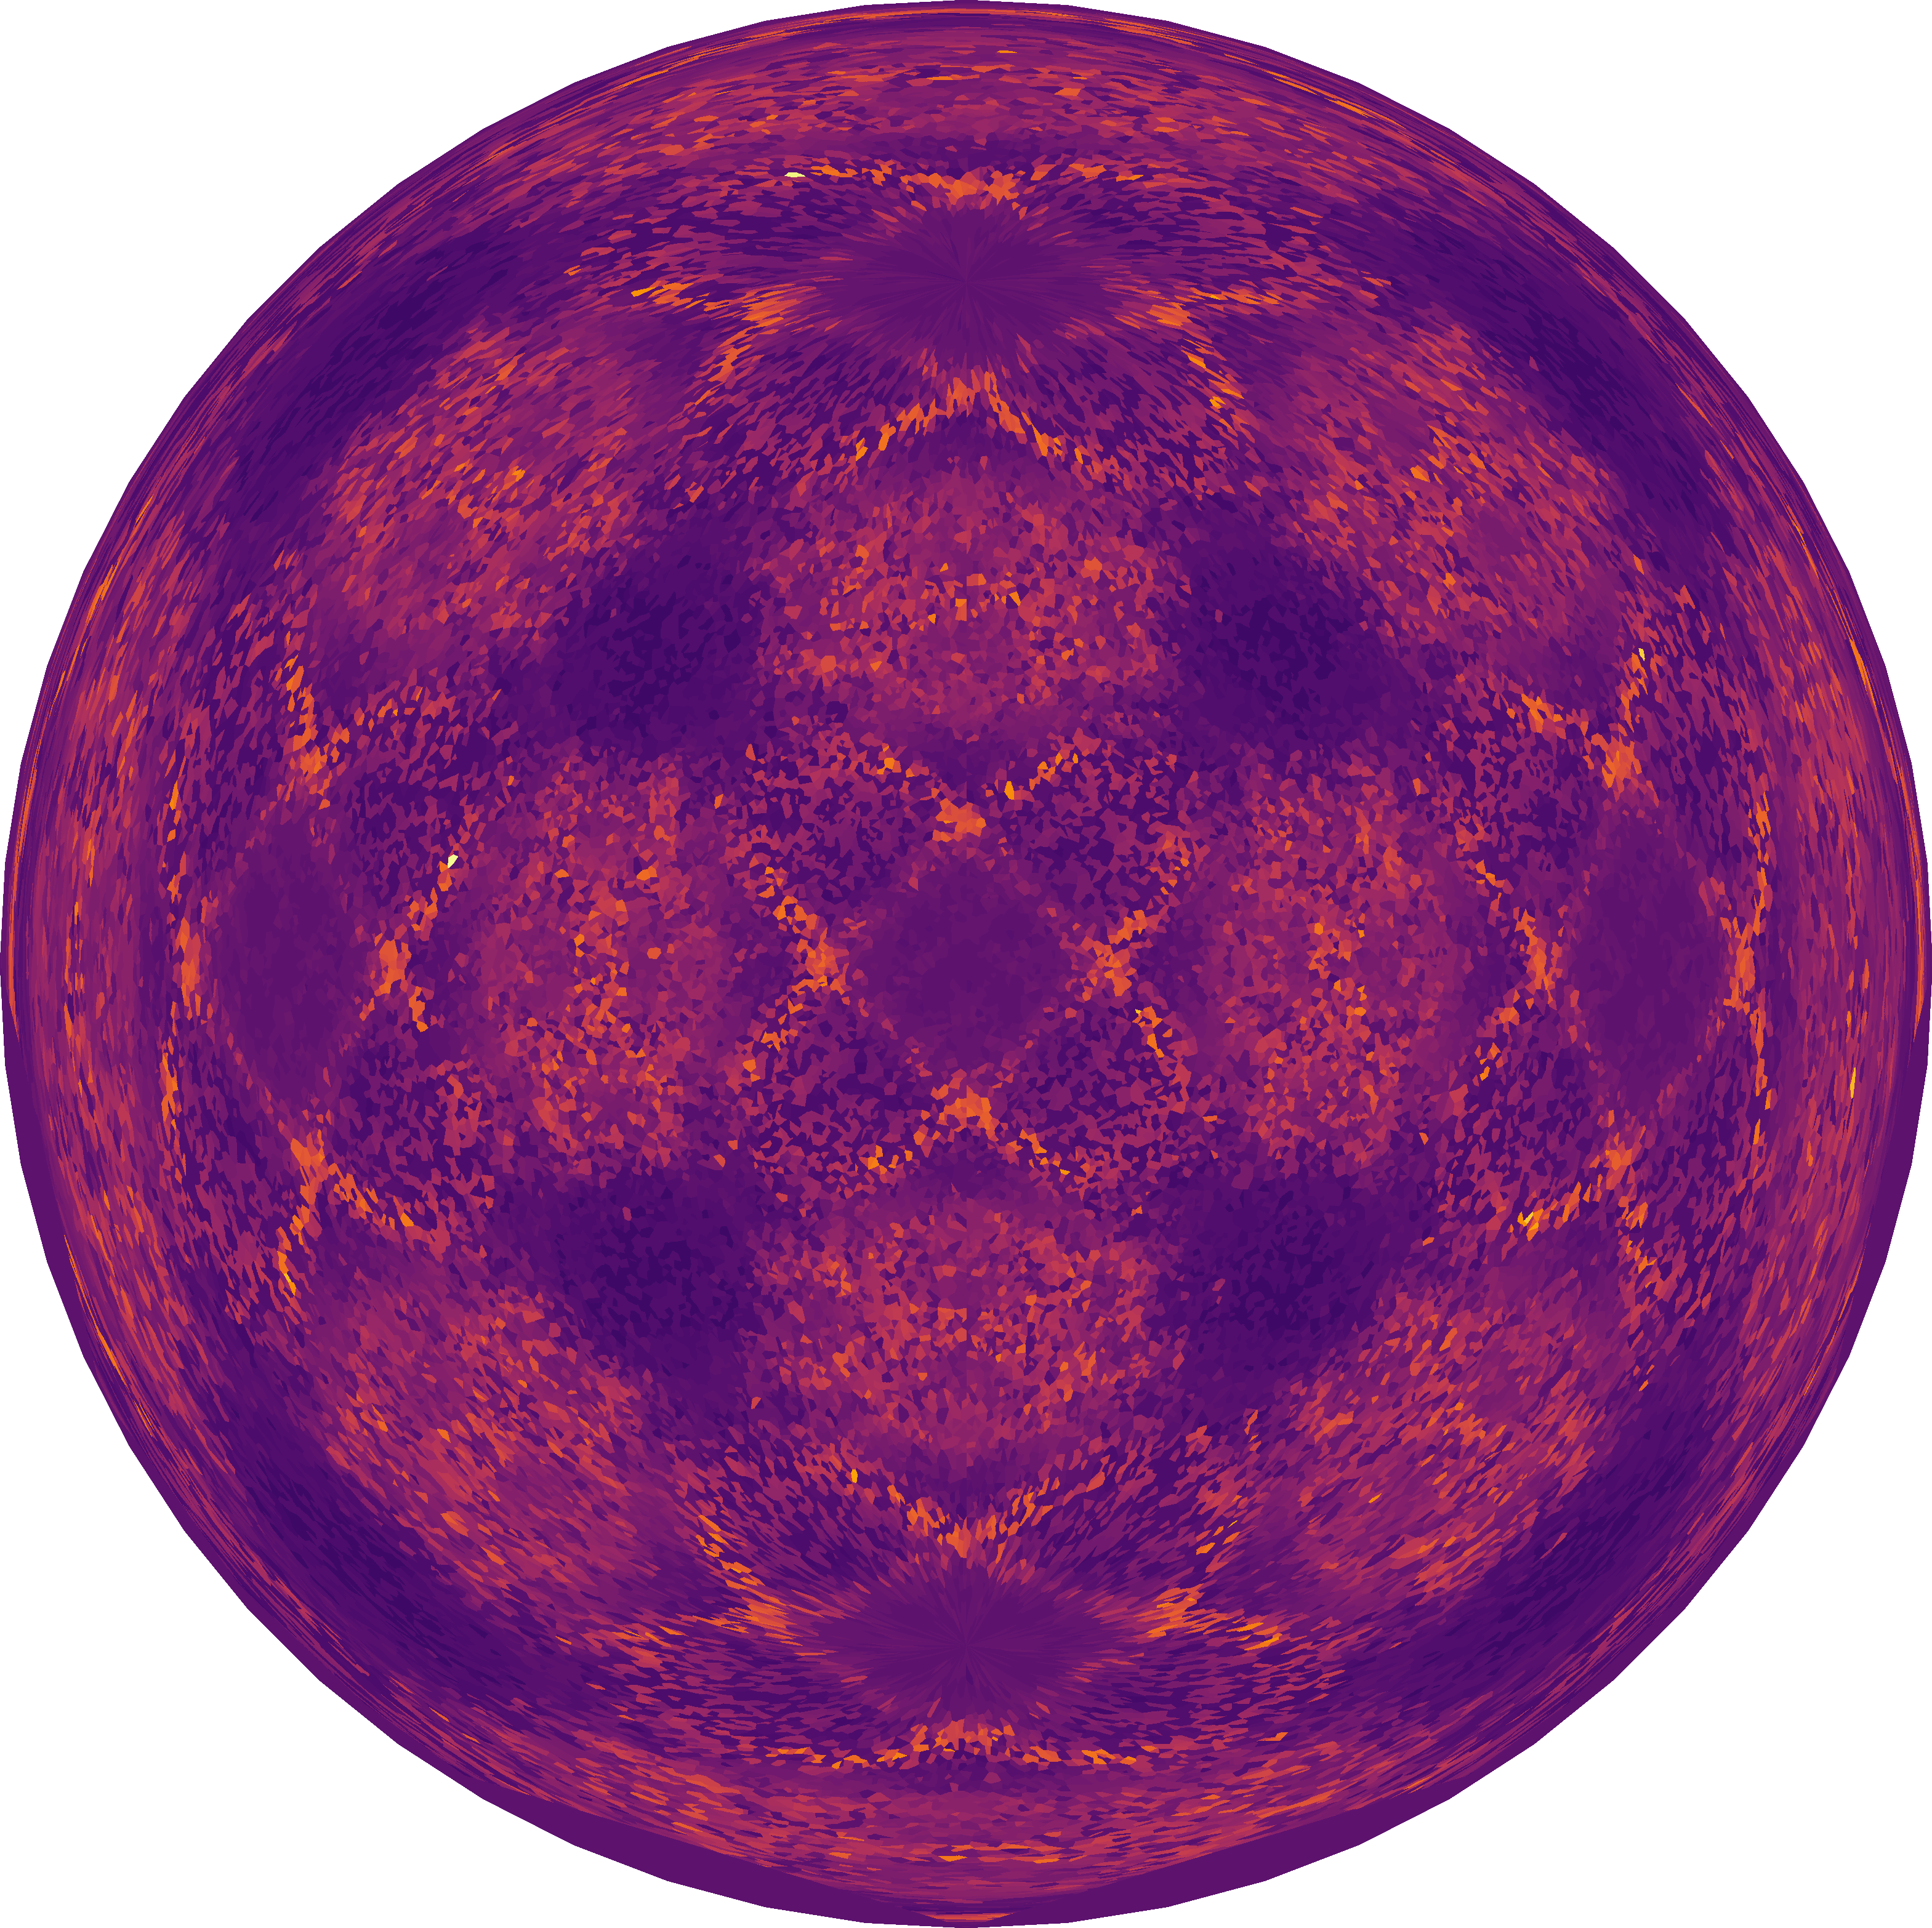
\includegraphics[width=0.95\textwidth]{surfaces/Ge_lambert_aea.png}
            };
            \addplot+ [mark = none, solid, color = \infernoaxiscolor]
                table {surfaces/horizontal_line_0.dat};
            \addplot+ [mark = none, solid, color = \infernoaxiscolor]
                table {surfaces/horizontal_line_1.dat};
            \addplot+ [mark = none, solid, color = \infernoaxiscolor]
                table {surfaces/horizontal_line_2.dat};
            \addplot+ [mark = none, solid, color = \infernoaxiscolor]
                table {surfaces/horizontal_line_3.dat};
            \addplot+ [mark = none, solid, color = \infernoaxiscolor]
                table {surfaces/horizontal_line_4.dat};
            \addplot+ [mark = none, solid, color = \infernoaxiscolor]
                table {surfaces/vertical_line_0.dat};
            \addplot+ [mark = none, solid, color = \infernoaxiscolor]
                table {surfaces/vertical_line_1.dat};
            \addplot+ [mark = none, solid, color = \infernoaxiscolor]
                table {surfaces/vertical_line_2.dat};
            \addplot+ [mark = none, solid, color = \infernoaxiscolor]
                table {surfaces/vertical_line_3.dat};
            \addplot+ [mark = none, solid, color = \infernoaxiscolor]
                table {surfaces/vertical_line_4.dat};
        \end{axis}
    \end{tikzpicture}
    \caption{High-resolution map of the threshold displacement energy surface for germanium based on around 86,000 randomly sampled directions from \textcite{KadribasicEtAl2018} displayed using a Lambert azimuthal equal-area projection.}
    \label{fig:ge-threshold-energy}
\end{figure}

\chapter{Dark matter velocity distributions and the laboratory frame}
\label{chap:dist}

The present understanding of the distribution of dark matter is (to a first approximation) that galaxies, such as the Milky Way, are situated inside a roughly spherically symmetric halo of dark matter moving at non-relativistic velocities following largely a Maxwellian velocity distribution stationary in the galactic frame. At a more granular level, substructures of local over and underdensities, streams, and other deviations from a spherical halo and Maxweillian velocity distribution are expected to exist. This general picture of the distribution of dark matter is formed from observations from galactic rotation curves \parencites{SofueEtAl1999, LelliMcGaughSchombert2016}, observations of structure of the Milky Way \parencites{PortailEtAl2016, LabiniEtAl2023, BelokurovEtAl2018, KruijssenEtAl2018, HelmiEtAl2018}, and simulations of structure formation \parencites{VogelsbergerEtAl2014, WangEtAl2015, KlypinEtAl2016, SpringelEtAl2017, SpringelEtAl2008, DiemandEtAl2008, StadelEtAl2009, vandenBoschOgiya2018}.

Although it is generally understood that the distribution of dark matter in the galactic halo tends to be spherically symmetric, its precise radial profile is less well known. The observed flattening of the galactic rotation curves implies that at large radial distances from the galactic center the density drops as $r^{-2}$. This conclusion follows from elementary Newtonian physics, as the circular velocity inside a spherically symmetric mass distribution at radius $r$ is given by $v(r)=(GM(r)/r)^{1/2}$, where $M(r)$ is the mass contained within the radius. The condition $v(r)=\text{const.}$ requires $M(r)\propto r$, which in the spherically symmetric case implies a density $\rho(r)=(4\pi r^2)^{-1}dM/dr\propto r^{-2}$. However, when it comes to the density at smaller radial distances, presently available observational data is compatible with a number of low-$r$ behaviors for the density profile. Plausible models for the density profile include those of \textcite{NavarroFrenkWhite1996}, Einasto \parencites{Einasto1965, MerrittEtAl2006}, \textcite{Burkert1995}, as well as the isothermal core profile \parencites{BahcallSoneira1980, BegemanBroeilsSanders1991}. Profiles can generally be divided into core profiles (isothermal core, Burkert), where the density profile flattens out at radii close to zero, and cuspy profiles which grow to a large value towards the galactic center (NFW, Einasto). It is worth noting that there exists tension between observations of galaxy rotation curves and galaxy formation over the shapes of the density profiles with observations preferring core profiles, while simulations prefer cuspy profiles. For discussion on this and other small scale structure issues, see this recent review by \textcite{TulinYu2018}.

Crucial from the point of view of direct detection experiments is the dark matter velocity distribution $f(\vec{v})$ as it in part determines the directional and energy distribution of scattering events in an experiment. Commonly, the velocity distribution of dark matter is taken to be the end state of a violent relaxation, which mixes the energies of the particles in a stochastic process \parencite{LyndenBell1967}. The distribution of velocities is then one which maximizes the entropy under energy conservation, i.e., the Maxwell--Boltzmann distribution $f(\vec{v})\propto \exp(-v^2/2\sigma^2)$. However, in the long term, particles whose velocities exceed the escape velocity of the halo will get ejected from the system. Taking into account this process leads to the standard halo model (SHM) velocity distribution
\begin{equation}
    f_{SHM}(\vec{v})\propto e^{-v^2/2\sigma^2}\Theta(v_\text{esc}-v).
    \label{eq:shm-dist}
\end{equation}

The standard halo model has traditionally been the velocity distribution assumed by the majority of direct detection studies because it is one of the few distributions for which~\eqref{eq:dm-master-rate} has nice closed form solutions. However, it is reasonable to expect the true velocity distribution to deviate from it in substantial ways. This is already somewhat evident from the abrupt cutoff at $v=v_\text{esc}$. Indeed, an ad-hoc model which removes the cutoff may be written as
\begin{equation}
    f(\vec{v})\propto(e^{-(v_\text{esc}^2-v^2)/2\sigma^2}-1)\Theta(v_\text{esc}-v).
\end{equation}
A generalization of this was given by \textcite{LisantiEtAl2011},
\begin{equation}
    f(\vec{v})\propto(e^{-(v_\text{esc}^2-v^2)/2k\sigma^2}-1)^k\Theta(v_\text{esc}-v),
\end{equation}
where a parameter value $k\in[1.5,3.5]$ was shown to fit the high velocity tail obtained from $N$-body simulations.

The velocity distributions discussed above all share the property of being isotropic. While isotropic distributions are computationally easier to handle, they are not motivated by $N$-body simulations or available data from the stellar neighborhood. Studies fitting separate radial and tangential parts
\begin{equation}
    f(v_r)\propto e^{-(v_r^2/2\sigma_r^2)^{\alpha_r}},\quad f(v_t)\propto v_te^{-(v_t^2/2\sigma_t^2)^{\alpha_t}},
\end{equation}
onto data from various $N$-body simulations have found that the velocity dispersion in the radial direction tends to be greater than in the tangential direction \parencites{FairbairnSchwetz2009, KuhlenEtAl2010}. Furthermore, recent analysis of data gathered by the Gaia satellite suggests the presence of a ``sausage'' structure, which has been suggested to be the result of a past galaxy merger event \parencites{BelokurovEtAl2018, KruijssenEtAl2018, HelmiEtAl2018}. This sausage exhibits significant anisotropy  in the velocity space, with its isosurfaces forming elongated shapes which give it its name. Based on this model, \textcite{EvansOHareMcCabe2019} suggest the $\text{SHM}^{++}$ velocity distribution
\begin{equation}
    f(\vec{v})=(1-\eta)f_R(\vec{v})+\eta f_S(\vec{v}),
\end{equation}
which consists of a round component $f_R(\vec{v})$ given by the SHM distribution~\eqref{eq:shm-dist} combined with a highly anisotropic sausage component
\begin{equation}
    f_S(\vec{v})\propto\exp\left(-\frac{v_r^2}{2\sigma_r^2}-\frac{v_\theta^2}{2\sigma_\theta^2}-\frac{v_\varphi^2}{2\sigma_\varphi^2}\right).
\end{equation}
Here $\sigma_r$ is the radial velocity dispersion as before, while $\sigma_\theta$ and $\sigma_\varphi$ are the tangential and azimuthal dispersions, respectively, relative to the galactic plane. As before, the tangential and azimuthal dispersions are taken to be degenerate such that $\sigma_\theta=\sigma_\varphi$.

Beyond the overall shape of the dark matter halo and its typical velocity distribution, the true local galactic environment is a complex dynamic environment. The Milky Way is surrounded by a number of smaller satellite galaxies, and their existence suggests the presence of subhalos of dark matter within the larger galactic halo. These subhalos can get torn apart by tidal forces, which lead to dark matter streams: structures of dark matter with overall velocity relative to the galactic center, and small velocity dispersion. Some observational evidence for dark matter streams comes from observations of the Sagittarius stream \parencite{BelokurovEtAl2013} and from recent Gaia data\parencite{NecibLisantiBelokurov2019}. However, numerical simulations suggest the existence of a large number of streams \needcite. Although streams constitute a small part of the total mass of the dark matter halo \needcite, they can form a significant contribution to the local density if one happens to be passing through the Earth.

\section{Earth's motion and the dark matter halo}

The dark matter halo, by definition, should have no overall linear motion in the galactic frame, because the galactic coordinate system is defined as stationary relative to the galactic center of mass. Then the motion of dark matter in any neighborhood should come from rotational motion of the halo. Indeed, the dark matter halo necessarily has some angular momentum. However, in the view where the galactic disk and dark matter halo formed from the same collapsing mass of baryons and dark matter, the rotational velocity of the halo should be negligible compared to that of the much more compact galactic disk. More formally, one can define the dimensionless spin parameter $\lambda=JE^{1/2}/GM^{5/2}$, where $J$, $E$ and $M$ are the total angular momentum, energy, and mass of the system, respectively, and $G$ is the gravitational constant. The spin parameter characterizes the portion of the system's energy stored in angular motion. Numerical simulations of galaxy formation find $\lambda_\text{disk}\gg\lambda_\text{halo}$, which supports the view that the rotational motion of the halo is small \parencites{MoMaoWhite1998, WarrenEtAl1992, KimmEtAl2011}. For this reason standard treatments of dark matter direct detection tend to neglect the rotational motion.

Attempts to observe scattering events of dark matter particles from the galactic halo are in the forseeable future likely to take place in terrestrial laboratories. From the observer's perspective then, regardless of what minor angular motion the halo has, the dark matter appears to be coming at us at the same speed with which Earth moves through the galaxy. The immediate consequence of this is that the mean of the velocity distribution gets shifted such that $f(\vec{v})\rightarrow f(\vec{v}+\vec{v}_\text{lab})$, where $\vec{v}_\text{lab}$ is the velocity of the laboratory frame relative to the galactic frame. In addition, relevant for direct detection experiments with any kind of sensitivity to the direction of the incoming dark matter particles is the orientation of the laboratory frame with respect to the galactic frame, which for any terrestrial frame is not constant due to the rotation of the Earth. Full understanding of these coordinate transformations is therefore imperative for prediction and interpretation of potential direct detection signals.

The composition of $\vec{v}_\text{lab}$ to well-understood components is straightforward. The greatest contribution comes from the rotational motion of the Milky Way galaxy, which gives for the mean motion of the local neighborhood of the solar system the circular velocity $\vec{v}_\text{circ}$ with an observed magnitude of around 220--240 km/s. The solar system has some peculiar motion relative to its surroundings, which introduces a correction $\vec{v}_\text{pec}$ to the velocity. The combination of these two velocities gives the center of mass velocity of the solar system. An observer on Earth then has two motions with respect to the rest frame of the solar system: the orbital velocity of Earth $\vec{v}_\text{orb}$ and rotational velocity of a point on the Earth's surface $\vec{v}_\text{rot}$ from the rotation of the Earth about its axis. Of these the orbital velocity $\vec{v}_\text{orb}$ has a magnitude around 30 km/s, and therefore has a significant contribution to $\vec{v}_\text{lab}$ which produces the well-known and sought for annual modulation of the dark matter direct detection signal. The magnitude of $\vec{v}_\text{rot}$ is at most about 0.46 km/s. In principle its presence causes a daily modulation of the direct detection signal via the same principle as the annual modulation signal, but because of its small amplitude this signal is unlikely to be detectable by any experiment in the foreseeable future. In any case $\vec{v}_\text{lab}$ may be written as
\begin{equation}
    \vec{v}_\text{lab}=\vec{v}_\text{circ}+\vec{v}_\text{pec}+\vec{v}_\text{orb}+\vec{v}_\text{rot}.
\end{equation}
It is useful to combine the two constant components $\vec{v}_\text{circ}$ and $\vec{v}_\text{pec}$ into a single component $\vec{v}_\text{sol}=\vec{v}_\text{circ}+\vec{v}_\text{pec}$, the velocity of the solar system in the galactic frame, such that
\begin{equation}
    \vec{v}_\text{lab}=\vec{v}_\text{sol}+\vec{v}_\text{orb}+\vec{v}_\text{rot}.
\end{equation}

\begin{table}
    \begin{tblr}[
        tall,
        caption = {Coordinate systems for transforming between the galactic frame and a lab frame.},
        label = {tab:coordsys},
        note{*} = {The axes as defined in the ICRS deviate from the J2000.0 north celestial pole and March equinox by $\sim0.01''$. This deviation is insignificant for this work and is neglected for sake of simplicity.},
        remark{Note} = {All coordinate systems are right-handed by convention and therefore completely defined by their $z$- and $x$-axes. The orientation of the DCS is not defined because it depends on the specifics of the detector type. The GCS is defined as being centered on the Sun at any given moment, but is defined to be stationary in the sense that it has no velocity relative to the galactic center. J2000.0 is the reference epoch for the ICRS axes.}]
    {
        colspec = {X[l]X[l]X[l]X[l]},
        hline{1,Z} = {0.08em},
        hline{2} = {0.05em}
    }
        Coordinate system & Center & $z$-direction & $x$-direction\\
        Galactic coordinate system (GCS) & Solar system barycenter & North galactic pole & Galactic center \\
        International Celestial Reference System (ICRS) & Solar system barycenter & North celestial pole (J2000.0)\TblrNote{*} & March equinox (J2000.0)\TblrNote{*} \\
        Horizontal coordinate system (HCS) & Detector & Zenith & North \\
        Detector coordinate system (DCS) & Detector & --- & ---\\
    \end{tblr}
\end{table}

The relevant coordinate system definitions for transforming between the laboratory frame and the galactic frame are summarized in table \ref{tab:coordsys}. The dark matter velocity distribution is first transformed from the galactic coordinate system (GCS) to the International Celestial Reference System (ICRS), which is the standard celestial coordinate reference system. The ICRS closely resembles the traditional equatorial coordinate system, but is defined to be nonrotating with respect to distant extragalactic radio sources, as defined by the International Earth Rotation and Reference Systems Service (IERS) \parencite{MaFeissel1997}. From the ICRS, to get to a frame corresponding to an Earth-based laboratory, a transformation is made to the horizontal coordinate system (HCS). From here a transformation is made to the detector coordinate system (DCS), which is the laboratory frame in which the dark matter scattering is described. The exact definition of the DCS is arbitrary, and depends on what is a useful coordinate system for describing the detector. In the case of a crystalline detector with a detection anisotropy that exhibits the symmetries of the crystal, for example, this might be a coordinate system whose axes are perpendicular to the walls of the crystals rectangular unit cell. The transformation between the HCS and DCS is then a rotation that depends on the exact orientation of the detector crystal. This would be relevant in the context of a specific detector, but in a generic theoretical analysis of detector concepts, no valuable insight is lost by assuming $\text{HCS}=\text{DCS}$.

For the purposes of this analysis, all transformations here are described as Galilean transformations consisting of a rotation $R$ and a boost $\vec{v}$ (the translational part of the transformation is not relevant for analysis of dark matter scattering).

Because of complexities arising from many-body interactions in the solar system, as well as from motions of the Earth's crust, precise definitions of the transformation between the ICRS and HCS involve various corrections of different orders of magnitude. Given that the present state of dark matter direct detection is that no experiment has observed a confirmed dark matter signal to begin with, that any potential observed signal would be weak and subject to large uncertainties, that existing directional detection technologies have poor angular resolution, and that there are significant uncertainties in the parameters of the GCS to ICRS transformation already, a highly accurate determination of the ICRS to HCS transformation is hardly necessary. Therefore, for the purposes of this work, we can safely ignore angular corrections that result in corrections significantly less than 1\degree{} per century or $40''$ per year.

\section{Coordinates: GCS to ICRS}

The galactic coordinate system (GCS) is defined as a coordinate system centered on the Sun, which has its $z$-axis perpendicular to the galactic plane, towards the galactic north pole, and its $x$-axis towards the galactic center. Although it is defined to be centered on the Sun at any given moment, it is defined to have no velocity relative to the galactic center, and therefore it functions as a rest frame for the dark matter halo. Its orientation relative to the ICRS is completely described by three observable angles: the right ascension $\alpha_\text{NGP}$ and declination $\delta_\text{NGP}$ of the north galactic pole, as well as the galactic longitude $\ell_\text{NCP}$ of the north celestial pole. The latter is expressed in galactic coordinates, but from figure~\ref{fig:galtrans} can be easily seen to be equal to the position angle of the galactic center. Recent observational values of these angles provided by \cite{KarimMamajek2017} are shown in table~\ref{tab:gcs}.

\begin{figure}
    \center
    \tdplotsetmaincoords{60}{-45}
    \newcommand{\galcolor}{\secondarylinecolor}
    \newcommand{\equcolor}{\primarylinecolor}
    \newcommand{\intercolor}{black}
    \newcommand{\fadecolor}{black!20!white}
    \begin{tikzpicture}[tdplot_main_coords, scale = 1.1]
        \draw [thick, ->, \equcolor]
            (0,0,0)--(3,0,0)node[anchor=south west]{$x$};
        \draw [thick, ->, \equcolor]
            (0,0,0)--(0,3,0)node[anchor=south east]{$y$};
        \draw [thick, ->, \equcolor]
            (0,0,0)--(0,0,3)node[anchor=south]{NCP};
        \draw [thick, dashed]
            (0,0,0)--(-2.605,-0.5892,0)--(-2.605,-0.5892,1.466);
        \tdplotdrawarc [\fadecolor] {(0,0,0)}{3}{0}{360}{}{};
        \tdplotdrawarc [thick, dashed] {(0,0,0)}{0.5}{0}{192.7}{anchor = south}{$\alpha_\text{NGP}$};
        \tdplotsetrotatedcoords{90}{90}{90};
        \tdplotdrawarc [thick, tdplot_rotated_coords, dashed]{(0,0,0)}{0.8}{0}{27.087}{anchor = north east}{$\delta_\text{NGP}$};
        %\tdplotsetrotatedcoords{0}{0}{192.7};
        %\draw[tdplot_rotated_coords,->](0,0,0)--(3,0,0)node[anchor=north]{$x''$};
        %\draw[tdplot_rotated_coords,->](0,0,0)--(0,3,0)node[anchor=east]{$y''$};
        %\draw[tdplot_rotated_coords,->](0,0,0)--(0,0,3)node[anchor=east]{$z''$};
        \tdplotsetrotatedcoords{12.7}{-62.916}{0};
        %\draw[thick,\intercolor,tdplot_rotated_coords,->](0,0,0)--(3,0,0)node[anchor=south]{$x'$};
        %\draw[thick,\intercolor,tdplot_rotated_coords,->](0,0,0)--(0,3,0)node[anchor=south east]{$y'$};
        \draw [thick,\galcolor,tdplot_rotated_coords,->]
            (0,0,0)--(0,0,3) node [anchor = east] {NGP};
        %\draw[thick,tdplot_rotated_coords,->](0,0,0)--(0,-3,0)node[anchor=north west]{\ascnode};
        \tdplotdrawarc [\fadecolor,thick,tdplot_rotated_coords]{(0,0,0)}{3}{0}{360}{}{};
        \tdplotsetrotatedcoords{12.7}{-62.916}{237.07};
        \draw [thick,\galcolor,tdplot_rotated_coords,->]
            (0,0,0)--(3,0,0) node [anchor = north] {GC};
        \draw [thick,\galcolor,tdplot_rotated_coords,->]
            (0,0,0)--(0,3,0) node [anchor = south west] {$y'$};
        %\tdplotdrawarc[thick,tdplot_rotated_coords,dashed]{(0,0,0)}{0.8}{0}{32.93}{anchor=north west}{$\ell_0$};
        \tdplotdrawarc [thick, tdplot_rotated_coords, dashed]{(0,0,0)}{0.6}{0}{122.93}{anchor=north west}{$\ell_\text{NCP}$};
        \tdplotsetrotatedcoords{102.7}{-90}{0};
        \tdplotdrawarc[\fadecolor, thick, tdplot_rotated_coords]{(0,0,0)}{3}{0}{360}{}{};
        \tdplotsetrotatedcoords{137.848}{-41.67}{0};
        \tdplotdrawarc[\fadecolor, thick, tdplot_rotated_coords]{(0,0,0)}{3}{0}{360}{}{};
        \tdplotsetrotatedcoords{12.7}{-62.916}{180};
        \coordinate (Shift) at (-2.605,-0.5892,1.466);
        \tdplotsetrotatedcoordsorigin{(Shift)}
        %\tdplotdrawarc[thick,tdplot_rotated_coords,dashed]{(0,0,0)}{0.4}{0}{-122.93}{anchor=north east}{PA};
    \end{tikzpicture}
    \caption{Comparison of the equatorial and galactic coordinate systems. Orange axes are the GCS axes, and the blue axes are the ICRS axes. The angles $\alpha_\text{NGP}$ and $\delta_\text{NGP}$ are the right ascension and declination of the north galactic pole, respectively. Special labeled directions are the north galactic pole (NGP), galactic center (GC), and north celestial pole (NCP). The angle $\ell_\text{NCP}$ is the galactic longitude of the north celestial pole.}
    \label{fig:galtrans}
\end{figure}

\begin{table}\center
    \begin{tblr}[
        tall,
        label = {tab:gcs},
        caption = {Values of quantities defining the galactic coordinate system.},
        remark{Sources} = {The values for the top three parameters are from \textcite{KarimMamajek2017}. The value of the peculiar velocity is the commonly used value from \textcite{SchonrichBinneyDehnen2010}. A compilation of alternative values are given by \textcite{Coskunoglu2011}. The local circular velocity is not precisely known, so a range containing commonly used values is given; see text for details.}]
    {
        hspan = default,
        colspec = {lXl},
        width = \linewidth,
        hline{1,Z} = {0.08em},
        hline{2} = {0.05em}
    }
        Parameter & Units & Value \\
        $\alpha_\text{NGP}$ & degrees & $192.729\pm0.035$\\
        $\delta_\text{NGP}$ & degrees & $27.084\pm0.023$\\
        $\ell_\text{NCP}$ & degrees & $122.928\pm0.016$\\
        $\vec{v}_\text{pec}$ & km/s & $(11.1^{+0.69}_{-0.75},12.24^{+0.47}_{-0.47},7.25^{+0.37}_{-0.36})$\\
        $v_\text{circ}$ & km/s & 220--240\\
    \end{tblr}
\end{table}

The three angles given completely specify the rotational part of the transformation: a clockwise rotation about the $z$-axis by $\ell_\text{NCP}$, followed by a clockwise rotation about the $y$-axis by $\tfrac{\pi}{2}-\delta_\text{NGP}$, and finally a counterclockwise rotation about the $z$-axis by $\alpha_\text{NGP}-\pi$. These correspond to the rotations
\begin{equation}
    R_{\text{GCS}\rightarrow\text{ICRS}}=R_Z(\alpha_\text{NGP}-\pi)R_Y(\delta_\text{NGP}-\tfrac{\pi}{2})R_Z(-\ell_\text{NCP}).
\end{equation}

The boost part of the GCS to ICRS transform is simply given by $\vec{v}_\text{circ}+\vec{v}_\text{pec}$. Here we define the $\vec{v}_\text{circ}$ in terms of its GCS coordinates as $(0,v_\text{circ},0)$. The values for $\vec{v}_\text{pec}$ and $v_\text{circ}$ in GCS coordinates are listed in table~\ref{tab:gcs}. The value of $\vec{v}_\text{pec}$ is not precisely known. The value listed in the table is from \textcite{SchonrichBinneyDehnen2010}. \textcite{Coskunoglu2011} list values obtained by other studies. For $v_\text{circ}$ some disagreement exists in the literature over its value, owing to uncertainties in modeling the rotation curve of the Milky Way \parencite{McMillanBinney2009}. Most dark matter literature historically uses the value 220 km/s, which is close to the value $218\pm6$ km/s reported by \textcite{Bovy2012}. However, recent analyses favor a value $233\pm3$ km/s \parencites{McMillan2017, EvansOHareMcCabe2019}.

\section{Coordinates: ICRS to DCS}

The transformation between ICRS and HCS is conceptually and computationally more complex than the transformation between GCS and ICRS, because it first involves a transformation into a frame that both travels and rotates with the Earth, and then a transformation to a frame that corresponds to an observer on the surface of the Earth, involving the relevant rotation and boost. The first part of the transformation is consists of a boost by the Earth's orbital velocity $\vec{v}_\text{orb}$. Computing it is an exercise in basic Keplerian orbits. The displacement vector of an orbiting body from the locus of the orbit in the orbital plane is given by
\begin{equation}
    \vec{r}(t)=(r(\nu(t))\cos\nu(t),r(\nu(t))\sin\nu(t)),
    \label{eq:keplerdisp}
\end{equation}
where
\begin{equation}
    r(\nu)=\frac{a(1-e^2)}{1+e\cos\nu},
\end{equation}
where $a$ is the semi-major axis of the orbit, $e$ is the orbital eccentricity, and $\nu(t)$ is the true anomaly of the orbit at time $t$. We can express equation~\eqref{eq:keplerdisp} in terms of the eccentric anomaly $E$ of the orbit via
\begin{equation}
    \cos\nu=\frac{\cos E-e}{1-e\cos E},\qquad\sin\nu=\frac{\sqrt{1-e^2}\sin E}{1-e\cos E},
\end{equation}
whose time dependent in turn can be computed from the mean anomaly $M=M_0+2\pi(t-t_0)$ via Kepler's equation
\begin{equation}
    E-e\sin E=M.
\end{equation}
Here $t_0$ is the epoch at which $M=M_0$. The orbital velocity is then straightforward to compute by differentiating equation~\eqref{eq:keplerdisp} and using conservation of orbital angular momentum to obtain
\begin{equation}
    \vec{v}_\text{orb}(t)=\left(-\frac{2\pi}{T}\frac{a}{\sqrt{1-e^2}}\sin\nu(t),\frac{2\pi}{T}\frac{a}{\sqrt{1-e^2}}(e+\cos\nu(t))\right),
    \label{eq:vorbkep}
\end{equation}
where $T$ is the orbital period.

The coordinates of equation~\eqref{eq:vorbkep} are given in the orbital plane, centered on the Sun, with the $x$-axis aligned in the direction of the perihelion. For purposes of performing the boost with this velocity, it needs to be expressed in the ICRS. The necessary rotation can be written in terms of the argument of perihelion $\omega$, the obliquity of the orbital plane $\bar{\phi}$, and longitude of ascending node $\Omega$ of the orbit at time $t$. These quantities evolve with time due to the precession of the orbital plane, but are below $50''$ per century, and it is therefore sufficient to assume the J2000.0 values. The value of $\Omega$ is approximately zero, so the relevant rotation is
\begin{equation}
    R_{\text{kep}\rightarrow\text{ICRS}}\approx R_X(\varepsilon_\text{J2000.0})R_Z(\omega_\text{J2000.0}).
\end{equation}

The boost by Earth's orbital velocity effectively takes us to the Geocentric Celestial Reference System (GCRS), which is a geocentric variant of the ICRS. The next step in the transformation procedure towards the HCS is an intermediate transformation to the International Terrestrial Reference System (ITRS), which is defined as a geocentric system having no rotation with respect to the Earth's surface. The transformation between the GCRS and ITRS is described in detail in the IERS Conventions \parencite{LuzumPetit2010}. The GCRS to ITRS transformation itself relies on two intermediate coordinate systems. First, the GCRS is transformed to the Celestial Intermediate Coordinate System (CIRS). The purpose of this transformation, and the CIRS, is to account for the precession and nutation of the Earth's axis. The transformation then proceeds to the Terrestrial Intermediate Coordinate System (TIRS), which rotates with the Earth. The transformation between the TIRS and ITRS accounts for the motion of the Earth's rotational axis relative to its crust (polar motion).

The precession, nutation, and polar motion are extremely small effects. The polar motion has a period on the order of years with an amplitude around $0.5''$, while the nutation components are on the order of arcseconds. The precession progresses slowly at a rate of tens of arcseconds per year, and is therefore its effect can be expected to not exceed multiple arcminutes over this century. Considering the present state of dark matter direct detection experiments, this level of accuracy in the coordinate system orientation is not necessary in any foreseeable future. Therefore, for our purposes, it is sufficient to only account for the rotation of the Earth, such that
\begin{equation}
    R_{\text{GRCS}\rightarrow\text{ITRS}}\approx R_Z(-\text{ERA}),
\end{equation}
where $ERA$ is the Earth rotation angle \parencite{LuzumPetit2010},
\begin{equation}
    \text{ERA}=2\pi(0.7790572732640+1.00273781191135448\cdot\text{UT1}_\text{J2000.0}).
\end{equation}
Here $\text{UT1}_\text{J2000.0}$ refers to the Universal Time defined with the origin $\text{UT1}_\text{J2000.0}=0$ on the J2000.0 epoch, January 1st, 2000, at 12:00 Terrestrial Time. UT1 is related to the Coordinated Universal Time (UTC) by $|\text{UT1}-\text{UTC}|<0.9$ s, which is ensured by the addition of leap seconds to UTC. For practical purposes one can therefore assume $\text{UT1}\approx\text{UTC}$.

From the ITRS, the coordinates are next rotated to the orientation of the HCS at some latitude $\lambda$ and longitude $\varphi$. To be precise, by definition of the $z$-axis of the HCS being defined by the zenith direction, the appropriate notion of latitude to use is the astronomical latitude, determined by the angle of local gravitational acceleration relative to the equatorial plane. However, the deviations of astronomical latitude from the geodetic latitude (angle of surface normal of the reference ellipsoid to the equatorial plane) are on the order of arcseconds, so geodetic latitude is sufficient. In any case, once the appropriate definition of latitude has been chosen, the corresponding rotation is given by
\begin{equation}
    R_{\text{ITRS}\rightarrow\text{HCS}}=R_Y(\tfrac{\pi}{2}-\lambda)R_Z(-\varphi).
\end{equation}
Once in the correct orientation, the coordinate system needs to be boosted eastward to account for the rotation of the Earth, i.e., with velocity $\vec{v}_\text{rot}=(0,-v_\text{rot},0)$. Since this is already a subdominant correction to the total velocity $\vec{v}_\text{lab}$, we may assume a spherical model of the Earth, in which case $v_\text{rot}=R_0\cos\lambda$, where $R_0$ denotes the mean radius of the Earth.

Without further specification of the detector setup, the transformation between the HCS and DCS may bee any general rotation matrix. Given the unit vectors $\unitv{x}_\text{DCS}$, $\unitv{y}_\text{DCS}$ and $\unitv{z}_\text{DCS}$ defining the axes of the DCS, expressed in HCS coordinates, this rotation matrix is
\begin{equation}
    R_{\text{HCS}\rightarrow\text{DCS}}=
    (
        \unitv{x}_\text{DCS},
        \unitv{y}_\text{DCS},
        \unitv{z}_\text{DCS}
    )^\transp.
\end{equation}
Appropriate definition of the DCS depends on the problem at hand. In general, the orientation of the coordinate system is only relevant if the detector has some known anisotropy that makes the signal sensitive to the orientation of the detector. The DCS should be defined in a manner which is both possible for an experiment to determine and relate to the HCS, and sufficiently unambiguous in the context of the theoretical description of the detector anisotropy. For example, in the context of anisotropy derived from the lattice structure of a cubic crystal the DCS axes could be the axes of the unit cell.

\section{Observational consequences of Earth's motion}

The motion of the Earth-based detector relative to the dark matter distribution shows on Earth as a dark matter wind hitting the Earth at velocity $\vec{v}_\text{DM}=-\vec{v}_\text{lab}$. In a hypothetical directional direct detection experiment this would imply the angular distribution of recoil events having a peak in the direction of $\vec{v}_\text{DM}$. This can be seen by considering equation~\eqref{eq:dm-master-rate} in the simple case of nucleon scattering with a $\tmean{|\mathcal{M}|^2}\sim 1$ interaction with an isotropic velocity distribution. The relevant part of the equation is
\begin{equation}
    \ddder{R_S}{E}{\Omega}\sim\int\delta\left(\vec{v}\cdot\unitv{q}+v_\text{min}\right)f(\vec{v}+\vec{v}_\text{lab})\difd^3v.
\end{equation}
A change of variables $\vec{v}'=\vec{v}+\vec{v}_\text{lab}$ in the integral and solution of the trivial angular part then gives
\begin{equation}
    \ddder{R_S}{E}{\Omega}\sim\int_{|\vec{v}_\text{lab}\cdot\unitv{q}+v_\text{min}|}^\infty vf(v)\difd v.
    \label{eq:isotropic-rate}
\end{equation}
Since $vf(v)$ is positive, the integral is monotonic as a function of the lower limit. Therefore, as a function of $v_\text{min}\sim E^{1/2}$, it reaches a maximum at $v_\text{min}=\max\{0,-\vec{v}_\text{lab}\cdot\unitv{q}\}$. It follows that the energy integrated event rate $dR_S/d\Omega$ is maximized when $-\vec{v}_\text{lab}\cdot\unitv{q}=v_\text{lab}$, i.e., when $\unitv{q}=-\unitv{v}_\text{lab}$.

Such an anisotropy, whose direction remains fixed relative to the distant stars, opposing the motion of the solar system through the galaxy, would be a smoking gun signal for direct detection of dark matter. However, present prospects for directional detection capabilities are not there yet, and therefore evidence of nonterrestrial origin of direct detection signals must be sought by other means.

In the absence of any directional sensitivity, it is evident from the above considerations that the total scattering rate $R_S$ is larger for larger magnitudes of $\vec{v}_\text{lab}$. Therefore, any modulation of the magnitude $v_\text{lab}$ gets translated into a modulation of $R_S$ whose maximum coincides with the maximum of $v_\text{lab}$. The primary modulation component comes from the term $\vec{v}_\text{sol}+\vec{v}_\text{orb}$, where $\vec{v}_\text{orb}$ rotates in the Earth's orbital plane. This leads to an annual modulation in the magnitude of $\vec{v}_\text{lab}$, and consequently in the scattering rate, with a maximum occurring in the summer. This annual modulation offers the most well-studied feature of the signal that would allow discrimination of a dark matter signal from other naturally occurring backgrounds, as other sources of annual modulation with the same phase are difficult, although not impossible, to come up with.

Observation of an annual modulation signal with the desired phase has famously been claimed by the DAMA/LIBRA experiment since the early 2000s, with a presently stated significance of $13.7\sigma$ \parencite{BernabeiEtAl2023}. However, other experiments built to test the results of DAMA/LIBRA, using the same NaI scintillator crystals, have not observed an annual modulation \parencites{DMIce2017, COSINE1002019, COSINE1002024, KIMS2019, ANAIS2024}. Furthermore, the best-fit region of the dark matter fit for the signal is ruled out by multiple other experiments as shown in figure~\ref{fig:dd-reach}.  These results are difficult to reconcile with a dark matter interpretation of the DAMA/LIBRA signal.

There is, in principle, also a daily modulation signal arising from the variation of the magnitude of $\vec{v}_\text{lab}$ when the rotational velocity $\vec{v}_\text{rot}$ of the detector on Earth's surface is taken into account. Given that the rotational velocity is, at its maximum around 0.46 km/s, this modulation is subdominant compared to the annual modulation. More common source of signal modulation, however, are anisotropies in the detector response. One can see that if equation~\eqref{eq:isotropic-rate} is multiplied by a direction dependent response factor $S(E,\unitv{q})$, whose orientation is fixed relative to the laboratory frame, then the effect the response factor has on the event rate varies as the Earth rotates about its axis, leading to a daily variation in the observed rate of events.

The daily modulation caused by detector response can be substantially more varied in nature than the annual modulation, or the daily modulation from variation of the magnitude $v_\text{lab}$. The latter two modulations generally have the same period as the motion that generates them: around 365 days (length of a sidereal year), and around 24 hours (length of a stellar day), respectively. However, the daily modulation due to the detector response, in general, consists of a combination of harmonics of the fundamental period of a stellar day. Depending on the shape of the detector response, and the orientation of the detector, any one of the harmonics may dominate, and therefore the dominant period of the modulation may also be half a stellar day, or third of a stellar day, or fourth of a stellar day, and so on.

A notable property of both types of daily modulation caused by the Earth's motion is that the phase of the signal varies throughout the year. Let $\vec{v}_E=\vec{v}_\text{sol}+\vec{v}_\text{orb}$ denote the center of mass velocity of Earth, and let $\vec{v}_E^\parallel$ be its component parallel to the equatorial plane. One period of daily modulation is then defined as the length of time it takes for the Earth to make one full revolution relative to $\vec{v}_E^\parallel$. If the direction of $\vec{v}_E^\parallel$ was constant, the daily modulation period would be exactly a stellar day. However, due to the time dependence of $\vec{v}_\text{orb}$, the direction of $\vec{v}_E^\parallel$ drifts throughout the year. This causes the period of daily modulation to vary slowly, which can be modeled as a time-dependent phase whose value is equal to the right ascension of the dark matter wind speed $\alpha_w(t)$. Neglecting the small effect of Earth's axial tilt relative to the orbital plane, it is straightforward to show that the magnitude of the phase variation is approximately given by
\begin{equation}
    \Delta\alpha_w\approx 2\arcsin\left(\frac{|\vec{v}_\text{orb}^\parallel|}{|\vec{v}_\text{sol}^\parallel|}\right),
\end{equation}
which has a value of around 20\degree.

There is similarly a variation in the declination of the dark matter wind speed, $\delta_w(t)$, which results from variation in the velocity component $\vec{v}_E^\perp$ perpendicular to the orbital plane. This variation, of around 15\degree{}, can be seen in figure~\ref{fig:v-lab-dir} showing the daily paths of the direction of $\vec{v}_\text{lab}$ and solar direction $\unitv{r}_\odot$ throughout the year as seen by an observer on Earth. This variation of the declination has the effect of slightly changing the profile of the daily modulation throughout the year.

Overall, the presence of these significant variations in both the declination and right ascension of the direction of $\vec{v}_\text{lab}$, in combination with the dependence of daily modulation on the orientation of the detector, makes the analysis of daily modulation substantially more complicated than the comparatively simple analysis of yearly modulation. Publication~\ref{pub:sassi2024} contains a detailed analysis on the variation in the daily modulation in germanium when the crystal orientation is changed. This analysis shows that the daily modulation can be dominated by completely different harmonics of the 24 hour period depending on the orientation of the crystal. That is, in one orientation the dominant period could be 12 hours, while in another it could be 6 hours. Furthermore, the dominant period depends on the degree of anisotropy in the velocity distribution. This complexity creates both challenges and opportunities. On one hand, the complex harmonic structure makes fitting daily modulation onto data far more difficult than in the case of annual modulation, and more assumptions are needed about the underlying model. On the other hand, the fact that daily modulation is senitive to the model means that it could be used to aid in model discrimination in the event of discovery of a signal.

\begin{figure}
    \center
    \begin{tikzpicture}
        \pgfplotsset{point meta min=1, point meta max=13.0}
        \begin{axis}[
                scale only axis = true,
                height = 0.99\textwidth,
                axis y line = none,
                axis x line = none,
                axis line style = {draw = white},
                title style = {at = {(0.5,0.9)}},
                width = 0.99\textwidth,
                ymin = -2.0,
                ymax = 2.0,
                xmin = -2.0,
                xmax = 2.0,
                every axis plot/.append style = {line width = 1.0pt},
                colormap name = twilight,
                colorbar,
                colorbar horizontal,
                colorbar style = {
                    at = {(0.5,-0.07)},
                    xlabel = Date,
                    xtick = {1, 2, 3, 4, 5, 6, 7, 8, 9, 10, 11, 12, 13},
                    xticklabels = {Jan, Feb, Mar, Apr, May, Jun, Jul, Aug, Sep, Oct, Nov, Dec, Jan},
                    width = 0.95*\pgfkeysvalueof{/pgfplots/parent axis width},
                    anchor = north},
                cycle list = {[samples of colormap = {13}]},
                name = border]
            \fill [color=\plotbgcolor]
                (axis cs:0,0) circle [radius = 2.0];
            \addlegendimage{no markers,grey};
            \label{legend.A};
            \addlegendimage{no markers,grey,dashed};
            \label{legend.B};
            \addplot+ [mark = none, solid, color = \plotfgcolor]
                table {surfaces/horizontal_line_0.dat};
            \addplot+ [mark = none, solid, color = \plotfgcolor]
                table {surfaces/horizontal_line_1.dat};
            \addplot+ [mark = none, solid, color = \plotfgcolor]
                table {surfaces/horizontal_line_2.dat};
            \addplot+ [mark = none, solid, color = \plotfgcolor]
                table {surfaces/horizontal_line_3.dat};
            \addplot+ [mark = none, solid, color = \plotfgcolor]
                table {surfaces/horizontal_line_4.dat};
            \addplot+ [mark = none, solid, color = \plotfgcolor]
                table {surfaces/vertical_line_0.dat};
            \addplot+ [mark = none, solid, color = \plotfgcolor]
                table {surfaces/vertical_line_1.dat};
            \addplot+ [mark = none, solid, color = \plotfgcolor]
                table {surfaces/vertical_line_2.dat};
            \addplot+ [mark = none, solid, color = \plotfgcolor]
                table {surfaces/vertical_line_3.dat};
            \addplot+ [mark = none, solid, color = \plotfgcolor]
                table {surfaces/vertical_line_4.dat};
            \pgfplotsset{cycle list shift = -10};
            \addplot+ [mark = none, solid]
                table {directions/dm_wind_dir_46.47186_-81.18669_2024-01-01_2024-01-01-23-50_lambert_aea.dat} -- cycle;
            \addplot+ [mark = none, solid]
                table {directions/dm_wind_dir_46.47186_-81.18669_2024-02-01_2024-02-01-23-50_lambert_aea.dat} -- cycle;
            \addplot+ [mark = none, solid]
                table {directions/dm_wind_dir_46.47186_-81.18669_2024-03-01_2024-03-01-23-50_lambert_aea.dat} -- cycle;
            \addplot+ [mark = none, solid]
                table {directions/dm_wind_dir_46.47186_-81.18669_2024-04-01_2024-04-01-23-50_lambert_aea.dat} -- cycle;
            \addplot+ [mark = none, solid]
                table {directions/dm_wind_dir_46.47186_-81.18669_2024-05-01_2024-05-01-23-50_lambert_aea.dat} -- cycle;
            \addplot+ [mark = none, solid]
                table {directions/dm_wind_dir_46.47186_-81.18669_2024-06-01_2024-06-01-23-50_lambert_aea.dat} -- cycle;
            \addplot+ [mark = none, solid]
                table {directions/dm_wind_dir_46.47186_-81.18669_2024-07-01_2024-07-01-23-50_lambert_aea.dat} -- cycle;
            \addplot+ [mark = none, solid]
                table {directions/dm_wind_dir_46.47186_-81.18669_2024-08-01_2024-08-01-23-50_lambert_aea.dat} -- cycle;
            \addplot+ [mark = none, solid]
                table {directions/dm_wind_dir_46.47186_-81.18669_2024-09-01_2024-09-01-23-50_lambert_aea.dat} -- cycle;
            \addplot+ [mark = none, solid]
                table {directions/dm_wind_dir_46.47186_-81.18669_2024-10-01_2024-10-01-23-50_lambert_aea.dat} -- cycle;
            \addplot+ [mark = none, solid]
                table {directions/dm_wind_dir_46.47186_-81.18669_2024-11-01_2024-11-01-23-50_lambert_aea.dat} -- cycle;
            \addplot+ [mark = none, solid]
                table {directions/dm_wind_dir_46.47186_-81.18669_2024-12-01_2024-12-01-23-50_lambert_aea.dat} -- cycle;
            \pgfplotsset{cycle list shift = -12};
            \addplot+ [mark = none, dashed]
                table {directions/sun_dir_46.47186_-81.18669_2024-01-01_2024-01-01-23-50_lambert_aea.dat} -- cycle;
            \addplot+ [mark = none, dashed]
                table {directions/sun_dir_46.47186_-81.18669_2024-02-01_2024-02-01-23-50_lambert_aea.dat} -- cycle;
            \addplot+ [mark = none, dashed]
                table {directions/sun_dir_46.47186_-81.18669_2024-03-01_2024-03-01-23-50_lambert_aea.dat} -- cycle;
            \addplot+ [mark = none, dashed]
                table {directions/sun_dir_46.47186_-81.18669_2024-04-01_2024-04-01-23-50_lambert_aea.dat} -- cycle;
            \addplot+ [mark = none, dashed]
                table {directions/sun_dir_46.47186_-81.18669_2024-05-01_2024-05-01-23-50_lambert_aea.dat} -- cycle;
            \addplot+ [mark = none, dashed]
                table {directions/sun_dir_46.47186_-81.18669_2024-06-01_2024-06-01-23-50_lambert_aea.dat} -- cycle;
            \addplot+ [mark = none, dashed]
                table {directions/sun_dir_46.47186_-81.18669_2024-07-01_2024-07-01-23-50_lambert_aea.dat} -- cycle;
            \addplot+ [mark = none, dashed]
                table {directions/sun_dir_46.47186_-81.18669_2024-08-01_2024-08-01-23-50_lambert_aea.dat} -- cycle;
            \addplot+ [mark = none, dashed]
                table {directions/sun_dir_46.47186_-81.18669_2024-09-01_2024-09-01-23-50_lambert_aea.dat} -- cycle;
            \addplot+ [mark = none, dashed]
                table {directions/sun_dir_46.47186_-81.18669_2024-10-01_2024-10-01-23-50_lambert_aea.dat} -- cycle;
            \addplot+ [mark = none, dashed]
                table {directions/sun_dir_46.47186_-81.18669_2024-11-01_2024-11-01-23-50_lambert_aea.dat} -- cycle;
            \addplot+ [mark = none, dashed]
                table {directions/sun_dir_46.47186_-81.18669_2024-12-01_2024-12-01-23-50_lambert_aea.dat} -- cycle;
            \node [
                    star,
                    star point ratio = 2.0,
                    scale = 0.5,
                    fill = \darkmarkcolor,
                    draw = \plotfgcolor,
                    thick] 
                at (0.000, 0.789) {};
            \node at (0.000, 0.789) [above right] {\small NCP};
        \end{axis}
        \newlength{\vlabdirwidth}
        \pgfextractx{\vlabdirwidth}{\pgfpointdiff{\pgfpointanchor{border}{west}}{\pgfpointanchor{border}{east}}}
        \addtolength{\vlabdirwidth}{-.696em}% inner sep
        \node[draw, below=3pt] at (border.south) {
            \begin{tblr}{
                hspan = minimal,
                rowsep = 0pt,
                colspec = {lX},
                width = 0.95\vlabdirwidth
            }
                \ref{legend.A} Incoming DM wind direction ($\unitv{v}_\text{lab}$) & \ref{legend.B} Solar direction ($\unitv{r}_\odot$) \\
            \end{tblr}
            %\makebox[0.95\vlabdirwidth]{\ref{legend.A} Incoming DM wind direction ($\unitv{v}_\text{lab}$)\hfil\ref{legend.B} Solar direction ($\unitv{r}_\odot$)}
        };
    \end{tikzpicture}
    \caption{Paths of the incoming dark matter wind direction (solid lines), and sun (dashed lines) on the first day of each month of the year 2024, as seen by a hypothetical observer at the location of the SNOLAB facility (46.47\degree N, 81.19\degree W) facing north, displayed using a Lambert azimuthal equal-area projection. The star marks the direction of the north celestial pole. The SNOLAB facility is the site of direct detection experiments from multiple collaborations, including \textcite{DEAP2016}, \textcite{PICO2016}, \textcite{SuperCDMS2017}, and \textcite{DAMIC2020}.}
    \label{fig:v-lab-dir}
\end{figure}

\chapter{Discussion}

\backmatter

\printbibliography[heading = bibintoc, title = References]

\end{document}
